\documentclass{article}

\usepackage{amsmath,amssymb,amsthm,mathtools}
\usepackage{physics}
\usepackage[left=1cm,right=1cm,top=1cm,bottom=2cm]{geometry}
\usepackage{pgfplots}
\usetikzlibrary{backgrounds}
\pgfplotsset{compat=newest}
\usepgfplotslibrary{fillbetween}

\newtheorem{example}{Příklad}
\newtheorem*{remark}{\underline{\it pozn.:}}

\makeatletter
\usepackage{xpatch}
\xpatchcmd{\@thm}{\thm@headpunct{.}}{\thm@headpunct{}}{}{}
\makeatother

\begin{document}
\fontsize{10pt}{15pt}\selectfont
\setcounter{example}{27}
\begin{example}
	Řešte metodou střelby Blasiovu rovnici mezní vrstvy
	\begin{gather*}
		y''' + y y'' + \lambda \left( 1 - y'^{2} \right)  = 0,
		\qq{kde } x \in (0,10) \qcomma \lambda \in \langle 0, 0.5 \rangle \\
		y(0) = y'(0) = 0 \qcomma y'(10) = 1
	\end{gather*}
	\smallskip
	\hrule
	\medskip
	Nejprve musíme diferenciální rovnici třetího řádu rozložit na tři obyčejné diferenciální rovnice prvního řádu. To provedeme substitucemi:
	\begin{equation}
		\label{substituce}
		y = z^{(0)}(x) \qcomma
		y' = z^{(1)}(x) = \dv{z^{(0)}}{x} \qcomma
		y'' = z^{(2)}(x) = \dv{z^{(1)}}{x} \qcomma
		y''' = z^{(3)}(x) = \dv{z^{(2)}}{x}.
	\end{equation}
	Dosazením \ref{substituce} do původní rovnice pak získáváme soustavu differenciálních rovnic prvního řádu pro funkce $z^{(0)}, z^{(1)}, z^{(2)}$:
	\begin{equation}
		\begin{aligned}
			z^{(0)}(x) & = y                                                                                   \\
			z^{(1)}(x) & = \dv{z^{(0)}}{x}                                                                     \\
			z^{(2)}(x) & = \dv{z^{(1)}}{x}                                                                     \\
			z^{(3)}(x) & = \dv{z^{(2)}}{x}(x) & = -\lambda \left( 1 - {z^{(1)}}^{2} \right)  - z^{(2)}z^{(0)}.
		\end{aligned}
	\end{equation}
	Počáteční podmínky se převedou na $z^{(0)}(0) = 0$ a $z^{(1)}(0) = 0$ a koncová podmínka na $z^{(1)}(10) = 1$.

	\medskip

	Tuto soustavu budeme vnímat jako vektorovou funkci od $x$, a definujeme $\vec{f}(x)$ jako její $\grad_x$ konkrétně
	\begin{equation}
		\vec{Z}(x) =
		\begin{pmatrix}
			z^{(0)}(x) \\
			z^{(1)}(x) \\
			z^{(2)}(x) \\
		\end{pmatrix} \qcomma
		\vec{f}\left(x,\vec{Z}\right) =
		\begin{pmatrix}
			\dv{z^{(0)}}{x}\eval_{x,\vec{Z}} \\
			\dv{z^{(1)}}{x}\eval_{x,\vec{Z}} \\
			\dv{z^{(2)}}{x}\eval_{x,\vec{Z}} \\
		\end{pmatrix}  =
		\begin{pmatrix}
			z^{(1)}(x,\vec{Z}) \\
			z^{(2)}(x,\vec{Z}) \\
			z^{(3)}(x,\vec{Z}) \\
		\end{pmatrix} =
		\begin{pmatrix}
			z^{(1)} \\
			z^{(2)} \\
			-\lambda \left( 1 - {z^{(1)}}^{2} \right)  - z^{(2)}z^{(0)}
		\end{pmatrix}.
	\end{equation}
	Numerické řešení budeme provádět jednosměrnou metodou střelby z bodu $x_{0} = \vec{0}$ a řešení diferenciálních rovnic s pokusnými počátečními podmínkami Rundge-Kutta metodou čtvrtého řádu tedy:
	\begin{equation}
		\begin{aligned}
			\vec{k}_{1} & = h \cdot \vec{f}\left(  x_{n}, \vec{Z}(x_{n}) \right)                                       \\
			\vec{k}_{2} & = h \cdot \vec{f}\left(  x_{n} + \frac{h}{2}, \vec{Z}(x_{n}) + \frac{\vec{k}_{1}}{2} \right) \\
			\vec{k}_{3} & = h \cdot \vec{f}\left( x_{n} + \frac{h}{2}, \vec{Z}(x_{n}) + \frac{\vec{k}_{2}}{2}  \right) \\
			\vec{k}_{4} & = h \cdot \vec{f}\left( x_{n} + h, \vec{Z}(x_{n}) + \vec{k}_{3}  \right)
		\end{aligned}
	\end{equation}
	kde finální tvar odhadu $\vec{Z}(x_{n+1})$ je
	\begin{equation}
		\vec{Z}(x_{n+1}) = \vec{Z}(x_{n}) + \frac{1}{6}  \left(\vec{k}_{1} +  2\vec{k}_{2} + 2\vec{k}_{3} + \vec{k}_{4} \right).
	\end{equation}
	Pro dopředný chod potřebujeme tři parametry v počátečním bodě a ty vezmeme jako
	\begin{equation}
		\vec{Z}(0) =
		\begin{pmatrix}
			z^{(0)}(0) \\
			z^{(1)}(0) \\
			z^{(2)}(0)
		\end{pmatrix},  \qq{přičemž} z^{(0)}(0) = z^{(1)}(0) = 0,
	\end{equation}
	tedy s našimi počátečními podmínkami hledáme v prostoru počátečních parametrů
	\begin{equation}
		\vec{Z}(0) \in \left(
		\begin{pmatrix}
			0 \\
			0 \\
			1 \\
		\end{pmatrix}
		\right)_{\lambda}.
	\end{equation}
	Koncový bod potom musí splňovat podmínku $z^{(1)}(10) = 1$, tedy koncové řešení je z prostoru
	\begin{equation}
		\vec{Z}(10) \in
		\begin{pmatrix}
			0 \\
			1 \\
			0 \\
		\end{pmatrix}  +
		\left(
		\begin{pmatrix}
			1 \\
			0 \\
			0 \\
		\end{pmatrix},
		\begin{pmatrix}
			0 \\
			0 \\
			1 \\
		\end{pmatrix}
		\right)_{\lambda}.
	\end{equation}
	Samotná střela potom probíhá tak, že začneme se dvěma zadanými počátečními podmínkami a jedním zvoleným algoritmem hledání kořene (viz. dále) v bodě $x = 0$ a vektor $\vec{Z}(0)$ zvoleným počtem kroků s pomocí Rundge-Kuttova předpisu pro změnu $\vec{Z}$ posouváme až do $\vec{Z}(10)$.
	\medskip
	K minimalizaci chyby splnění koncové podmínky, které je ekvivalentní hledání kořene funkce $B_{2}$ od $\vec{Z}_{0}$
	\begin{equation}
		B_{2}(x, \vec{Z}_{0}) \eval_{x = 10}= B_{2}(x, z^{(2)}_{0}) \eval_{x=0}= z^{(1)}(x) - 1 \eval_{x=10}= 0
	\end{equation}
	zkusíme použít naivní Newtonovou-Raphsonovou metodou. Přičemž pro vyhodnocení $z^{(1)}(10) - 1$ musíme vždy najít hodnotu $z^{(1)}(10)$ střelbou s proměnným počátečním parametrem $z^{(2)}_{0}$.

	\smallskip

	Protože máme prostor počátečních parametrů pouze jednodimenzionální, budeme k tomu potřebovat pouze parciální derivaci
	\begin{equation}
		\pdv{B_{2}}{z^{(2)}_{0}} \approx \frac{B_{2}(z^{(2)}_{0} + \Delta z^{(2)}_{0}) - B_{2}(z^{(2)}_{0})}{\Delta z^{(2)}_{0}}.
	\end{equation}
	Ta se získá dvěma střelami s počátečními parametry $z^{(2)}_{0} + \Delta z^{(2)}_{0}$ a $z^{(2)}_{0}$ pro vyhodnocení $z^{(1)}(x)\eval_{x=10} \eqqcolon z^{(1)}_{10}$ a následným vyhodnocením chybové funkce $B_{2}$.

	\bigskip

	Implementací se ukázalo, že naivní Newtonova-Raphsonova metoda na hledání kořene není vhodná, jelikož není v tomto příkladu zjevně stabilní. Při splnění koncové podmínky se totiž blíží parciální derivace $B_{2}$ podle $z^{(2)}_{0}$ nule neboli $\pdv{z^{(1)}_{10}}{z^{(2)}_{0}}$ = 0. Řešení je tedy v bodě extrému $B_{2}$ nebo v inflexním bodě s nulovou derivací. Tam naivní Newtonova-Raphsonova metoda na hledání kořene fungovat nebude.
	\begin{remark}
		Ekvivalentní příklad by bylo pro případ extrému hledání kořen paraboly $y(x) = ax^2\qcomma a \neq 0$ a pro případ inflexního bodu s nulovou derivací hledání kořene kubického monomu $y(x) = ax^3\qcomma a \neq 0$, kde není zaručeno, že interval omezující přítomnost kořene se zachová v jednotlivých iteracích.
	\end{remark}

	Tyto dva případy se ještě liší v tom, jakou metodu budeme moci pro hledání kořene využít. Pokud se jedná o případ, že je v bodě $z^{(2)}_{0}$ pouze inflexní bod, budeme schopni použít například metodu půlení intervalu, která je v tomto případě relativně rychlá protože vyžaduje malý počet numericky náročných vyhodnocení střel. Jelikož jistě z tvaru $f(x, \vec{Z})$ platí $\lim_{z^{(2)}_{0} \to \infty} B_{2}(10) < 0$ a z testování implementace vyšlo, že existují i počáteční hodnoty s kladnou hodnotou chybové funkce $B_{2}$ (například, $z^{(2)}_{0} = 0$), je dobrá šance, že tato metoda bude na příklad fungovat.

	\begin{remark}
		Mohli bychom použít metodu sečen, která konverguje rychleji, ale pro využití metody sečen by bylo nutné ve vhodnou chvíli přepnout na jinou metodu, jelikož pokud bychom chtěli přesný výsledek, bude nám na malých intervalech vznikat numerická chyba díky dělení rozdílem funkčních hodnot na krajích intervalu.

		(Nejsem si jistý, jestli toto by byl problém, vzhledem k tomu, že dělíme jistě menší hodnotu. Je možné, že numerická chyba převáží a výsledek bude větší než 1 tedy bod ležet mimo interval?)

		(Díky této numerické chybě je opět porušená záruka, že interval z další iterace je podmnožinou intervalu z předchozí iterace? Musela by se implementovat mezipaměť mezi jednotlivými iteracemi a logika, pro porušení této podmínky.)
	\end{remark}

	Co se týká implementace půlení intervalu, tak v pro zvolený interval, $(a,b)$, který obsahuje kořen vždy vyhodnotíme funkci (střelu) v $ c \coloneqq \frac{(a+b)}{2} = z^{(2)}_{0}$ a poté jeden z bodů $a,b$ nahradíme $c$, tak aby ve výsledném intervalu zůstal kořen (aby vyčíslení funkce na hranicích intervalu měli opačné znaménko).\pagebreak

	\section*{Výsledky}
	Grafické výsledky

    \begin{figure}[h]
	\centering
    \def\svgwidth{\textwidth}
	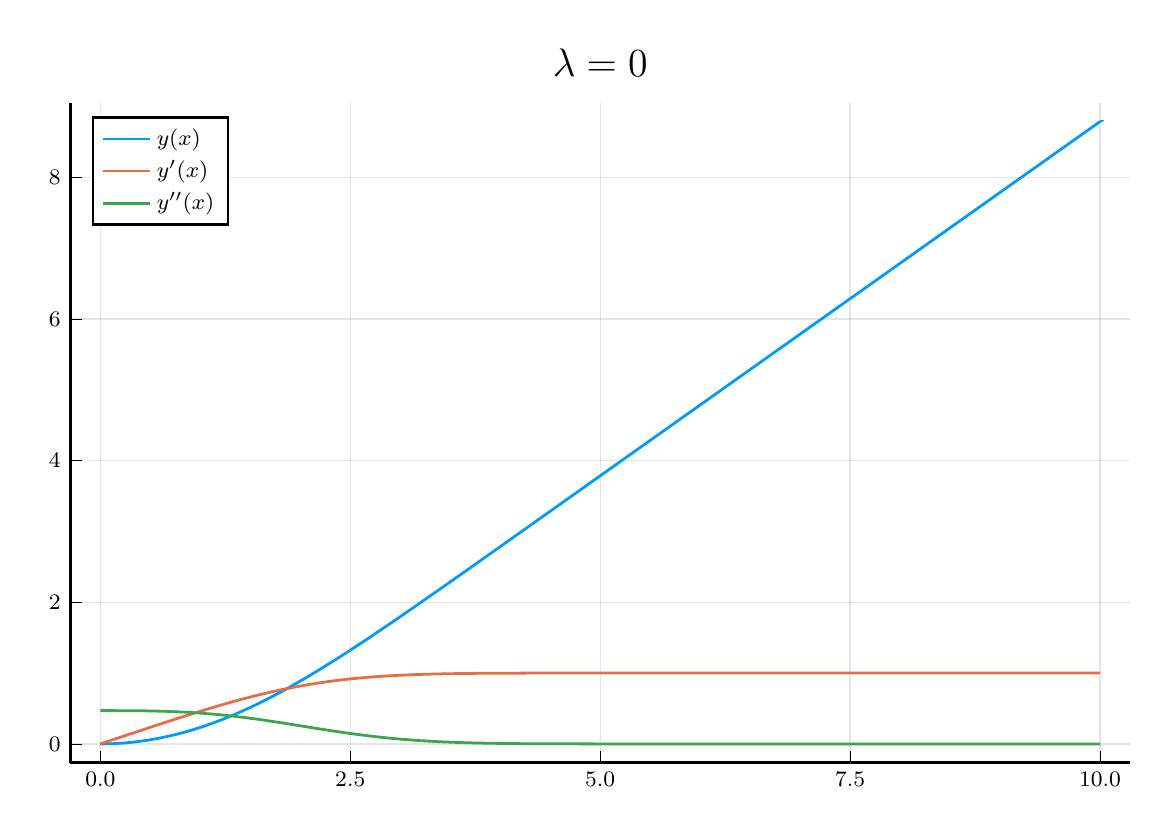
\begin{tikzpicture}[/tikz/background rectangle/.style={fill={rgb,1:red,1.0;green,1.0;blue,1.0}, draw opacity={1.0}}, show background rectangle]
\begin{axis}[point meta max={nan}, point meta min={nan}, legend cell align={left}, title={$\lambda = 0$}, title style={at={{(0.5,1)}}, anchor={south}, font={{\fontsize{14 pt}{18.2 pt}\selectfont}}, color={rgb,1:red,0.0;green,0.0;blue,0.0}, draw opacity={1.0}, rotate={0.0}}, legend style={color={rgb,1:red,0.0;green,0.0;blue,0.0}, draw opacity={1.0}, line width={1}, solid, fill={rgb,1:red,1.0;green,1.0;blue,1.0}, fill opacity={1.0}, text opacity={1.0}, font={{\fontsize{8 pt}{10.4 pt}\selectfont}}, text={rgb,1:red,0.0;green,0.0;blue,0.0}, at={(0.02, 0.98)}, anchor={north west}}, axis background/.style={fill={rgb,1:red,1.0;green,1.0;blue,1.0}, opacity={1.0}}, anchor={north west}, xshift={1.0mm}, yshift={-1.0mm}, width={150.4mm}, height={99.6mm}, scaled x ticks={false}, xlabel={}, x tick style={color={rgb,1:red,0.0;green,0.0;blue,0.0}, opacity={1.0}}, x tick label style={color={rgb,1:red,0.0;green,0.0;blue,0.0}, opacity={1.0}, rotate={0}}, xlabel style={at={(ticklabel cs:0.5)}, anchor=near ticklabel, font={{\fontsize{11 pt}{14.3 pt}\selectfont}}, color={rgb,1:red,0.0;green,0.0;blue,0.0}, draw opacity={1.0}, rotate={0.0}}, xmajorgrids={true}, xmin={-0.30000402}, xmax={10.300138019999999}, xtick={{0.0,2.5,5.0,7.5,10.0}}, xticklabels={{$0.0$,$2.5$,$5.0$,$7.5$,$10.0$}}, xtick align={inside}, xticklabel style={font={{\fontsize{8 pt}{10.4 pt}\selectfont}}, color={rgb,1:red,0.0;green,0.0;blue,0.0}, draw opacity={1.0}, rotate={0.0}}, x grid style={color={rgb,1:red,0.0;green,0.0;blue,0.0}, draw opacity={0.1}, line width={0.5}, solid}, axis x line*={left}, x axis line style={color={rgb,1:red,0.0;green,0.0;blue,0.0}, draw opacity={1.0}, line width={1}, solid}, scaled y ticks={false}, ylabel={}, y tick style={color={rgb,1:red,0.0;green,0.0;blue,0.0}, opacity={1.0}}, y tick label style={color={rgb,1:red,0.0;green,0.0;blue,0.0}, opacity={1.0}, rotate={0}}, ylabel style={at={(ticklabel cs:0.5)}, anchor=near ticklabel, font={{\fontsize{11 pt}{14.3 pt}\selectfont}}, color={rgb,1:red,0.0;green,0.0;blue,0.0}, draw opacity={1.0}, rotate={0.0}}, ymajorgrids={true}, ymin={-0.26362832999999997}, ymax={9.05123933}, ytick={{0.0,2.0,4.0,6.0,8.0}}, yticklabels={{$0$,$2$,$4$,$6$,$8$}}, ytick align={inside}, yticklabel style={font={{\fontsize{8 pt}{10.4 pt}\selectfont}}, color={rgb,1:red,0.0;green,0.0;blue,0.0}, draw opacity={1.0}, rotate={0.0}}, y grid style={color={rgb,1:red,0.0;green,0.0;blue,0.0}, draw opacity={0.1}, line width={0.5}, solid}, axis y line*={left}, y axis line style={color={rgb,1:red,0.0;green,0.0;blue,0.0}, draw opacity={1.0}, line width={1}, solid}, colorbar={false}]
    \addplot[color={rgb,1:red,0.0;green,0.6056;blue,0.9787}, name path={2fe807bc-4f14-44bc-8c52-e743dadf0dbf}, draw opacity={1.0}, line width={1}, solid]
        table[row sep={\\}]
        {
            \\
            0.0  0.0  \\
            0.01  2.3e-5  \\
            0.02  9.4e-5  \\
            0.03  0.000211  \\
            0.04  0.000376  \\
            0.05  0.000587  \\
            0.06  0.000846  \\
            0.07  0.001151  \\
            0.08  0.001504  \\
            0.09  0.001903  \\
            0.1  0.00235  \\
            0.11  0.002843  \\
            0.12  0.003383  \\
            0.13  0.003971  \\
            0.14  0.004605  \\
            0.15  0.005287  \\
            0.16  0.006015  \\
            0.17  0.00679  \\
            0.18  0.007613  \\
            0.19  0.008482  \\
            0.2  0.009398  \\
            0.21  0.010361  \\
            0.22  0.011371  \\
            0.23  0.012429  \\
            0.24  0.013533  \\
            0.25  0.014684  \\
            0.26  0.015882  \\
            0.27  0.017126  \\
            0.28  0.018418  \\
            0.29  0.019757  \\
            0.3  0.021143  \\
            0.31  0.022575  \\
            0.32  0.024054  \\
            0.33  0.025581  \\
            0.34  0.027154  \\
            0.35  0.028774  \\
            0.36  0.030441  \\
            0.37  0.032154  \\
            0.38  0.033915  \\
            0.39  0.035722  \\
            0.4  0.037576  \\
            0.41  0.039477  \\
            0.42  0.041424  \\
            0.43  0.043418  \\
            0.44  0.045459  \\
            0.45  0.047547  \\
            0.46  0.049681  \\
            0.47  0.051862  \\
            0.48  0.05409  \\
            0.49  0.056364  \\
            0.5  0.058684  \\
            0.51  0.061052  \\
            0.52  0.063465  \\
            0.53  0.065925  \\
            0.54  0.068432  \\
            0.55  0.070985  \\
            0.56  0.073585  \\
            0.57  0.07623  \\
            0.58  0.078922  \\
            0.59  0.081661  \\
            0.6  0.084446  \\
            0.61  0.087276  \\
            0.62  0.090153  \\
            0.63  0.093076  \\
            0.64  0.096046  \\
            0.65  0.099061  \\
            0.66  0.102122  \\
            0.67  0.105229  \\
            0.68  0.108382  \\
            0.69  0.111581  \\
            0.7  0.114826  \\
            0.71  0.118117  \\
            0.72  0.121453  \\
            0.73  0.124835  \\
            0.74  0.128262  \\
            0.75  0.131735  \\
            0.76  0.135253  \\
            0.77  0.138817  \\
            0.78  0.142426  \\
            0.79  0.146081  \\
            0.8  0.149781  \\
            0.81  0.153525  \\
            0.82  0.157315  \\
            0.83  0.16115  \\
            0.839999  0.16503  \\
            0.849999  0.168955  \\
            0.859999  0.172924  \\
            0.869999  0.176939  \\
            0.879999  0.180997  \\
            0.889999  0.185101  \\
            0.899999  0.189249  \\
            0.909999  0.193441  \\
            0.919999  0.197678  \\
            0.929999  0.201958  \\
            0.939999  0.206283  \\
            0.949999  0.210652  \\
            0.959999  0.215065  \\
            0.969999  0.219522  \\
            0.979999  0.224023  \\
            0.989999  0.228567  \\
            0.999999  0.233155  \\
            1.009999  0.237786  \\
            1.019999  0.24246  \\
            1.029999  0.247178  \\
            1.039999  0.251939  \\
            1.049999  0.256743  \\
            1.059999  0.261591  \\
            1.069999  0.26648  \\
            1.079999  0.271413  \\
            1.089999  0.276388  \\
            1.099999  0.281406  \\
            1.109999  0.286466  \\
            1.119999  0.291568  \\
            1.129999  0.296712  \\
            1.139999  0.301899  \\
            1.149999  0.307127  \\
            1.159999  0.312397  \\
            1.169999  0.317709  \\
            1.179999  0.323062  \\
            1.189999  0.328456  \\
            1.199999  0.333892  \\
            1.209999  0.339368  \\
            1.219999  0.344886  \\
            1.229999  0.350445  \\
            1.239999  0.356044  \\
            1.249999  0.361683  \\
            1.259999  0.367364  \\
            1.269999  0.373084  \\
            1.279999  0.378844  \\
            1.289999  0.384644  \\
            1.299999  0.390484  \\
            1.309999  0.396364  \\
            1.319999  0.402283  \\
            1.329999  0.408242  \\
            1.339999  0.414239  \\
            1.349999  0.420276  \\
            1.359999  0.426351  \\
            1.369999  0.432465  \\
            1.379999  0.438618  \\
            1.389999  0.444809  \\
            1.399999  0.451038  \\
            1.409999  0.457305  \\
            1.419999  0.46361  \\
            1.429999  0.469952  \\
            1.439999  0.476332  \\
            1.449999  0.48275  \\
            1.459999  0.489204  \\
            1.469999  0.495695  \\
            1.479999  0.502223  \\
            1.489999  0.508788  \\
            1.499999  0.515389  \\
            1.509999  0.522026  \\
            1.519999  0.528699  \\
            1.529999  0.535408  \\
            1.539999  0.542153  \\
            1.549999  0.548933  \\
            1.559999  0.555749  \\
            1.569999  0.562599  \\
            1.579999  0.569484  \\
            1.589999  0.576404  \\
            1.599999  0.583359  \\
            1.609999  0.590347  \\
            1.619999  0.59737  \\
            1.629999  0.604427  \\
            1.639999  0.611517  \\
            1.649999  0.618641  \\
            1.659999  0.625798  \\
            1.669999  0.632988  \\
            1.679999  0.640211  \\
            1.689999  0.647466  \\
            1.699999  0.654754  \\
            1.709999  0.662074  \\
            1.719999  0.669426  \\
            1.729999  0.67681  \\
            1.739999  0.684226  \\
            1.749999  0.691673  \\
            1.759999  0.699151  \\
            1.769999  0.70666  \\
            1.779999  0.714199  \\
            1.789999  0.721769  \\
            1.799999  0.72937  \\
            1.809999  0.737  \\
            1.819999  0.744661  \\
            1.829999  0.75235  \\
            1.839999  0.76007  \\
            1.849999  0.767818  \\
            1.859999  0.775596  \\
            1.869999  0.783402  \\
            1.879999  0.791237  \\
            1.889999  0.799099  \\
            1.899999  0.80699  \\
            1.909999  0.814909  \\
            1.919999  0.822856  \\
            1.929999  0.83083  \\
            1.939999  0.838831  \\
            1.949998  0.846858  \\
            1.959998  0.854913  \\
            1.969998  0.862994  \\
            1.979998  0.871102  \\
            1.989998  0.879235  \\
            1.999998  0.887394  \\
            2.009999  0.895579  \\
            2.019999  0.903789  \\
            2.029999  0.912024  \\
            2.039999  0.920285  \\
            2.049999  0.928569  \\
            2.059999  0.936879  \\
            2.069999  0.945212  \\
            2.079998  0.953569  \\
            2.089998  0.961951  \\
            2.099998  0.970355  \\
            2.109998  0.978783  \\
            2.119998  0.987235  \\
            2.129998  0.995709  \\
            2.139998  1.004205  \\
            2.149998  1.012724  \\
            2.159998  1.021265  \\
            2.169998  1.029829  \\
            2.179998  1.038413  \\
            2.189998  1.04702  \\
            2.199998  1.055647  \\
            2.209998  1.064296  \\
            2.219998  1.072966  \\
            2.229998  1.081656  \\
            2.239998  1.090367  \\
            2.249998  1.099097  \\
            2.259998  1.107848  \\
            2.269998  1.116619  \\
            2.279998  1.125409  \\
            2.289998  1.134218  \\
            2.299998  1.143046  \\
            2.309998  1.151894  \\
            2.319998  1.160759  \\
            2.329998  1.169644  \\
            2.339998  1.178546  \\
            2.349998  1.187467  \\
            2.359998  1.196405  \\
            2.369998  1.205361  \\
            2.379998  1.214334  \\
            2.389998  1.223325  \\
            2.399998  1.232332  \\
            2.409998  1.241357  \\
            2.419998  1.250398  \\
            2.429998  1.259455  \\
            2.439998  1.268528  \\
            2.449998  1.277617  \\
            2.459998  1.286722  \\
            2.469998  1.295843  \\
            2.479998  1.304978  \\
            2.489998  1.314129  \\
            2.499998  1.323295  \\
            2.509998  1.332476  \\
            2.519998  1.341671  \\
            2.529998  1.350881  \\
            2.539998  1.360104  \\
            2.549998  1.369342  \\
            2.559998  1.378594  \\
            2.569998  1.387859  \\
            2.579998  1.397137  \\
            2.589998  1.406429  \\
            2.599998  1.415734  \\
            2.609998  1.425051  \\
            2.619998  1.434382  \\
            2.629998  1.443724  \\
            2.639998  1.453079  \\
            2.649998  1.462447  \\
            2.659998  1.471826  \\
            2.669998  1.481217  \\
            2.679998  1.49062  \\
            2.689998  1.500034  \\
            2.699998  1.509459  \\
            2.709998  1.518896  \\
            2.719998  1.528343  \\
            2.729998  1.537801  \\
            2.739998  1.54727  \\
            2.749998  1.556749  \\
            2.759998  1.566239  \\
            2.769998  1.575739  \\
            2.779998  1.585248  \\
            2.789998  1.594768  \\
            2.799998  1.604297  \\
            2.809998  1.613835  \\
            2.819998  1.623383  \\
            2.829998  1.632941  \\
            2.839998  1.642507  \\
            2.849998  1.652082  \\
            2.859998  1.661666  \\
            2.869998  1.671259  \\
            2.879998  1.68086  \\
            2.889998  1.690469  \\
            2.899998  1.700086  \\
            2.909998  1.709712  \\
            2.919998  1.719346  \\
            2.929998  1.728987  \\
            2.939998  1.738636  \\
            2.949998  1.748293  \\
            2.959998  1.757957  \\
            2.969998  1.767628  \\
            2.979998  1.777306  \\
            2.989998  1.786991  \\
            2.999998  1.796684  \\
            3.009998  1.806383  \\
            3.019998  1.816088  \\
            3.029998  1.8258  \\
            3.039998  1.835519  \\
            3.049998  1.845244  \\
            3.059998  1.854975  \\
            3.069998  1.864712  \\
            3.079998  1.874455  \\
            3.089998  1.884204  \\
            3.099998  1.893959  \\
            3.109998  1.903719  \\
            3.119998  1.913485  \\
            3.129997  1.923256  \\
            3.139997  1.933032  \\
            3.149997  1.942814  \\
            3.159997  1.952601  \\
            3.169997  1.962393  \\
            3.179997  1.97219  \\
            3.189997  1.981991  \\
            3.199997  1.991797  \\
            3.209997  2.001608  \\
            3.219997  2.011424  \\
            3.229997  2.021244  \\
            3.239997  2.031068  \\
            3.249997  2.040897  \\
            3.259997  2.05073  \\
            3.269997  2.060566  \\
            3.279997  2.070407  \\
            3.289997  2.080252  \\
            3.299997  2.090101  \\
            3.309997  2.099953  \\
            3.319997  2.109809  \\
            3.329997  2.119669  \\
            3.339997  2.129533  \\
            3.349997  2.139399  \\
            3.359997  2.14927  \\
            3.369997  2.159143  \\
            3.379997  2.16902  \\
            3.389997  2.1789  \\
            3.399997  2.188783  \\
            3.409997  2.198669  \\
            3.419997  2.208559  \\
            3.429997  2.218451  \\
            3.439997  2.228345  \\
            3.449997  2.238243  \\
            3.459997  2.248143  \\
            3.469997  2.258047  \\
            3.479997  2.267952  \\
            3.489997  2.277861  \\
            3.499997  2.287771  \\
            3.509997  2.297685  \\
            3.519997  2.3076  \\
            3.529997  2.317518  \\
            3.539997  2.327438  \\
            3.549997  2.337361  \\
            3.559997  2.347286  \\
            3.569997  2.357212  \\
            3.579997  2.367141  \\
            3.589997  2.377072  \\
            3.599997  2.387005  \\
            3.609997  2.396939  \\
            3.619997  2.406876  \\
            3.629997  2.416814  \\
            3.639997  2.426754  \\
            3.649997  2.436697  \\
            3.659997  2.44664  \\
            3.669997  2.456586  \\
            3.679997  2.466533  \\
            3.689997  2.476481  \\
            3.699997  2.486431  \\
            3.709997  2.496383  \\
            3.719997  2.506336  \\
            3.729997  2.51629  \\
            3.739997  2.526246  \\
            3.749997  2.536204  \\
            3.759997  2.546162  \\
            3.769997  2.556122  \\
            3.779997  2.566083  \\
            3.789997  2.576046  \\
            3.799997  2.58601  \\
            3.809997  2.595975  \\
            3.819997  2.605941  \\
            3.829997  2.615908  \\
            3.839997  2.625876  \\
            3.849997  2.635845  \\
            3.859997  2.645815  \\
            3.869997  2.655787  \\
            3.879997  2.665759  \\
            3.889997  2.675732  \\
            3.899997  2.685707  \\
            3.909997  2.695682  \\
            3.919997  2.705657  \\
            3.929997  2.715634  \\
            3.939997  2.725612  \\
            3.949997  2.73559  \\
            3.959997  2.74557  \\
            3.969997  2.75555  \\
            3.979997  2.76553  \\
            3.989997  2.775512  \\
            3.999997  2.785494  \\
            4.009997  2.795477  \\
            4.019997  2.80546  \\
            4.029997  2.815444  \\
            4.039998  2.825429  \\
            4.049998  2.835415  \\
            4.059998  2.845401  \\
            4.069998  2.855387  \\
            4.079998  2.865374  \\
            4.089999  2.875362  \\
            4.099999  2.88535  \\
            4.109999  2.895339  \\
            4.119999  2.905328  \\
            4.13  2.915318  \\
            4.14  2.925308  \\
            4.15  2.935299  \\
            4.16  2.94529  \\
            4.170001  2.955282  \\
            4.180001  2.965274  \\
            4.190001  2.975266  \\
            4.200001  2.985259  \\
            4.210001  2.995252  \\
            4.220002  3.005245  \\
            4.230002  3.015239  \\
            4.240002  3.025234  \\
            4.250002  3.035228  \\
            4.260003  3.045223  \\
            4.270003  3.055218  \\
            4.280003  3.065214  \\
            4.290003  3.07521  \\
            4.300004  3.085206  \\
            4.310004  3.095202  \\
            4.320004  3.105199  \\
            4.330004  3.115196  \\
            4.340004  3.125193  \\
            4.350005  3.13519  \\
            4.360005  3.145188  \\
            4.370005  3.155186  \\
            4.380005  3.165184  \\
            4.390006  3.175182  \\
            4.400006  3.185181  \\
            4.410006  3.195179  \\
            4.420006  3.205178  \\
            4.430007  3.215178  \\
            4.440007  3.225177  \\
            4.450007  3.235177  \\
            4.460007  3.245177  \\
            4.470007  3.255177  \\
            4.480008  3.265177  \\
            4.490008  3.275177  \\
            4.500008  3.285177  \\
            4.510008  3.295178  \\
            4.520009  3.305179  \\
            4.530009  3.31518  \\
            4.540009  3.325181  \\
            4.550009  3.335182  \\
            4.560009  3.345183  \\
            4.57001  3.355184  \\
            4.58001  3.365186  \\
            4.59001  3.375187  \\
            4.60001  3.385189  \\
            4.610011  3.395191  \\
            4.620011  3.405193  \\
            4.630011  3.415195  \\
            4.640011  3.425197  \\
            4.650012  3.435199  \\
            4.660012  3.445202  \\
            4.670012  3.455204  \\
            4.680012  3.465207  \\
            4.690012  3.475209  \\
            4.700013  3.485212  \\
            4.710013  3.495214  \\
            4.720013  3.505217  \\
            4.730013  3.51522  \\
            4.740014  3.525223  \\
            4.750014  3.535226  \\
            4.760014  3.545229  \\
            4.770014  3.555232  \\
            4.780015  3.565235  \\
            4.790015  3.575239  \\
            4.800015  3.585242  \\
            4.810015  3.595245  \\
            4.820015  3.605249  \\
            4.830016  3.615252  \\
            4.840016  3.625256  \\
            4.850016  3.635259  \\
            4.860016  3.645263  \\
            4.870017  3.655267  \\
            4.880017  3.66527  \\
            4.890017  3.675274  \\
            4.900017  3.685278  \\
            4.910017  3.695282  \\
            4.920018  3.705286  \\
            4.930018  3.715289  \\
            4.940018  3.725293  \\
            4.950018  3.735297  \\
            4.960019  3.745301  \\
            4.970019  3.755305  \\
            4.980019  3.765309  \\
            4.990019  3.775313  \\
            5.00002  3.785317  \\
            5.01002  3.795321  \\
            5.02002  3.805326  \\
            5.03002  3.81533  \\
            5.04002  3.825334  \\
            5.050021  3.835338  \\
            5.060021  3.845343  \\
            5.070021  3.855347  \\
            5.080021  3.865351  \\
            5.090022  3.875355  \\
            5.100022  3.88536  \\
            5.110022  3.895364  \\
            5.120022  3.905368  \\
            5.130023  3.915373  \\
            5.140023  3.925377  \\
            5.150023  3.935381  \\
            5.160023  3.945386  \\
            5.170023  3.95539  \\
            5.180024  3.965395  \\
            5.190024  3.975399  \\
            5.200024  3.985404  \\
            5.210024  3.995408  \\
            5.220025  4.005413  \\
            5.230025  4.015417  \\
            5.240025  4.025422  \\
            5.250025  4.035426  \\
            5.260026  4.045431  \\
            5.270026  4.055435  \\
            5.280026  4.06544  \\
            5.290026  4.075444  \\
            5.300026  4.085449  \\
            5.310027  4.095453  \\
            5.320027  4.105458  \\
            5.330027  4.115462  \\
            5.340027  4.125467  \\
            5.350028  4.135471  \\
            5.360028  4.145476  \\
            5.370028  4.15548  \\
            5.380028  4.165485  \\
            5.390028  4.175489  \\
            5.400029  4.185494  \\
            5.410029  4.195498  \\
            5.420029  4.205503  \\
            5.430029  4.215508  \\
            5.44003  4.225512  \\
            5.45003  4.235517  \\
            5.46003  4.245521  \\
            5.47003  4.255526  \\
            5.480031  4.26553  \\
            5.490031  4.275535  \\
            5.500031  4.285539  \\
            5.510031  4.295544  \\
            5.520031  4.305548  \\
            5.530032  4.315553  \\
            5.540032  4.325557  \\
            5.550032  4.335562  \\
            5.560032  4.345566  \\
            5.570033  4.355571  \\
            5.580033  4.365575  \\
            5.590033  4.37558  \\
            5.600033  4.385584  \\
            5.610034  4.395589  \\
            5.620034  4.405593  \\
            5.630034  4.415598  \\
            5.640034  4.425602  \\
            5.650034  4.435607  \\
            5.660035  4.445611  \\
            5.670035  4.455616  \\
            5.680035  4.465621  \\
            5.690035  4.475625  \\
            5.700036  4.48563  \\
            5.710036  4.495634  \\
            5.720036  4.505639  \\
            5.730036  4.515643  \\
            5.740036  4.525648  \\
            5.750037  4.535652  \\
            5.760037  4.545657  \\
            5.770037  4.555661  \\
            5.780037  4.565666  \\
            5.790038  4.57567  \\
            5.800038  4.585675  \\
            5.810038  4.595679  \\
            5.820038  4.605684  \\
            5.830039  4.615688  \\
            5.840039  4.625693  \\
            5.850039  4.635697  \\
            5.860039  4.645702  \\
            5.870039  4.655706  \\
            5.88004  4.665711  \\
            5.89004  4.675715  \\
            5.90004  4.68572  \\
            5.91004  4.695724  \\
            5.920041  4.705729  \\
            5.930041  4.715734  \\
            5.940041  4.725738  \\
            5.950041  4.735743  \\
            5.960042  4.745747  \\
            5.970042  4.755752  \\
            5.980042  4.765756  \\
            5.990042  4.775761  \\
            6.000042  4.785765  \\
            6.010043  4.79577  \\
            6.020043  4.805774  \\
            6.030043  4.815779  \\
            6.040043  4.825783  \\
            6.050044  4.835788  \\
            6.060044  4.845792  \\
            6.070044  4.855797  \\
            6.080044  4.865801  \\
            6.090044  4.875806  \\
            6.100045  4.88581  \\
            6.110045  4.895815  \\
            6.120045  4.905819  \\
            6.130045  4.915824  \\
            6.140046  4.925828  \\
            6.150046  4.935833  \\
            6.160046  4.945837  \\
            6.170046  4.955842  \\
            6.180047  4.965847  \\
            6.190047  4.975851  \\
            6.200047  4.985856  \\
            6.210047  4.99586  \\
            6.220047  5.005865  \\
            6.230048  5.015869  \\
            6.240048  5.025874  \\
            6.250048  5.035878  \\
            6.260048  5.045883  \\
            6.270049  5.055887  \\
            6.280049  5.065892  \\
            6.290049  5.075896  \\
            6.300049  5.085901  \\
            6.31005  5.095905  \\
            6.32005  5.10591  \\
            6.33005  5.115914  \\
            6.34005  5.125919  \\
            6.35005  5.135923  \\
            6.360051  5.145928  \\
            6.370051  5.155932  \\
            6.380051  5.165937  \\
            6.390051  5.175941  \\
            6.400052  5.185946  \\
            6.410052  5.195951  \\
            6.420052  5.205955  \\
            6.430052  5.21596  \\
            6.440053  5.225964  \\
            6.450053  5.235969  \\
            6.460053  5.245973  \\
            6.470053  5.255978  \\
            6.480053  5.265982  \\
            6.490054  5.275987  \\
            6.500054  5.285991  \\
            6.510054  5.295996  \\
            6.520054  5.306  \\
            6.530055  5.316005  \\
            6.540055  5.326009  \\
            6.550055  5.336014  \\
            6.560055  5.346018  \\
            6.570055  5.356023  \\
            6.580056  5.366027  \\
            6.590056  5.376032  \\
            6.600056  5.386036  \\
            6.610056  5.396041  \\
            6.620057  5.406045  \\
            6.630057  5.41605  \\
            6.640057  5.426054  \\
            6.650057  5.436059  \\
            6.660058  5.446064  \\
            6.670058  5.456068  \\
            6.680058  5.466073  \\
            6.690058  5.476077  \\
            6.700058  5.486082  \\
            6.710059  5.496086  \\
            6.720059  5.506091  \\
            6.730059  5.516095  \\
            6.740059  5.5261  \\
            6.75006  5.536104  \\
            6.76006  5.546109  \\
            6.77006  5.556113  \\
            6.78006  5.566118  \\
            6.790061  5.576122  \\
            6.800061  5.586127  \\
            6.810061  5.596131  \\
            6.820061  5.606136  \\
            6.830061  5.61614  \\
            6.840062  5.626145  \\
            6.850062  5.636149  \\
            6.860062  5.646154  \\
            6.870062  5.656158  \\
            6.880063  5.666163  \\
            6.890063  5.676167  \\
            6.900063  5.686172  \\
            6.910063  5.696177  \\
            6.920063  5.706181  \\
            6.930064  5.716186  \\
            6.940064  5.72619  \\
            6.950064  5.736195  \\
            6.960064  5.746199  \\
            6.970065  5.756204  \\
            6.980065  5.766208  \\
            6.990065  5.776213  \\
            7.000065  5.786217  \\
            7.010066  5.796222  \\
            7.020066  5.806226  \\
            7.030066  5.816231  \\
            7.040066  5.826235  \\
            7.050066  5.83624  \\
            7.060067  5.846244  \\
            7.070067  5.856249  \\
            7.080067  5.866253  \\
            7.090067  5.876258  \\
            7.100068  5.886262  \\
            7.110068  5.896267  \\
            7.120068  5.906271  \\
            7.130068  5.916276  \\
            7.140069  5.92628  \\
            7.150069  5.936285  \\
            7.160069  5.94629  \\
            7.170069  5.956294  \\
            7.180069  5.966299  \\
            7.19007  5.976303  \\
            7.20007  5.986308  \\
            7.21007  5.996312  \\
            7.22007  6.006317  \\
            7.230071  6.016321  \\
            7.240071  6.026326  \\
            7.250071  6.03633  \\
            7.260071  6.046335  \\
            7.270072  6.056339  \\
            7.280072  6.066344  \\
            7.290072  6.076348  \\
            7.300072  6.086353  \\
            7.310072  6.096357  \\
            7.320073  6.106362  \\
            7.330073  6.116366  \\
            7.340073  6.126371  \\
            7.350073  6.136375  \\
            7.360074  6.14638  \\
            7.370074  6.156384  \\
            7.380074  6.166389  \\
            7.390074  6.176394  \\
            7.400074  6.186398  \\
            7.410075  6.196403  \\
            7.420075  6.206407  \\
            7.430075  6.216412  \\
            7.440075  6.226416  \\
            7.450076  6.236421  \\
            7.460076  6.246425  \\
            7.470076  6.25643  \\
            7.480076  6.266434  \\
            7.490077  6.276439  \\
            7.500077  6.286443  \\
            7.510077  6.296448  \\
            7.520077  6.306452  \\
            7.530077  6.316457  \\
            7.540078  6.326461  \\
            7.550078  6.336466  \\
            7.560078  6.34647  \\
            7.570078  6.356475  \\
            7.580079  6.366479  \\
            7.590079  6.376484  \\
            7.600079  6.386488  \\
            7.610079  6.396493  \\
            7.62008  6.406497  \\
            7.63008  6.416502  \\
            7.64008  6.426507  \\
            7.65008  6.436511  \\
            7.66008  6.446516  \\
            7.670081  6.45652  \\
            7.680081  6.466525  \\
            7.690081  6.476529  \\
            7.700081  6.486534  \\
            7.710082  6.496538  \\
            7.720082  6.506543  \\
            7.730082  6.516547  \\
            7.740082  6.526552  \\
            7.750082  6.536556  \\
            7.760083  6.546561  \\
            7.770083  6.556565  \\
            7.780083  6.56657  \\
            7.790083  6.576574  \\
            7.800084  6.586579  \\
            7.810084  6.596583  \\
            7.820084  6.606588  \\
            7.830084  6.616592  \\
            7.840085  6.626597  \\
            7.850085  6.636601  \\
            7.860085  6.646606  \\
            7.870085  6.65661  \\
            7.880085  6.666615  \\
            7.890086  6.67662  \\
            7.900086  6.686624  \\
            7.910086  6.696629  \\
            7.920086  6.706633  \\
            7.930087  6.716638  \\
            7.940087  6.726642  \\
            7.950087  6.736647  \\
            7.960087  6.746651  \\
            7.970088  6.756656  \\
            7.980088  6.76666  \\
            7.990088  6.776665  \\
            8.000088  6.786669  \\
            8.010088  6.796674  \\
            8.020088  6.806678  \\
            8.030088  6.816683  \\
            8.040089  6.826687  \\
            8.050089  6.836692  \\
            8.060089  6.846696  \\
            8.070089  6.856701  \\
            8.08009  6.866705  \\
            8.09009  6.87671  \\
            8.10009  6.886714  \\
            8.11009  6.896719  \\
            8.12009  6.906723  \\
            8.130091  6.916728  \\
            8.140091  6.926733  \\
            8.150091  6.936737  \\
            8.160091  6.946742  \\
            8.170092  6.956746  \\
            8.180092  6.966751  \\
            8.190092  6.976755  \\
            8.200092  6.98676  \\
            8.210093  6.996764  \\
            8.220093  7.006769  \\
            8.230093  7.016773  \\
            8.240093  7.026778  \\
            8.250093  7.036782  \\
            8.260094  7.046787  \\
            8.270094  7.056791  \\
            8.280094  7.066796  \\
            8.290094  7.0768  \\
            8.300095  7.086805  \\
            8.310095  7.096809  \\
            8.320095  7.106814  \\
            8.330095  7.116818  \\
            8.340096  7.126823  \\
            8.350096  7.136827  \\
            8.360096  7.146832  \\
            8.370096  7.156837  \\
            8.380096  7.166841  \\
            8.390097  7.176846  \\
            8.400097  7.18685  \\
            8.410097  7.196855  \\
            8.420097  7.206859  \\
            8.430098  7.216864  \\
            8.440098  7.226868  \\
            8.450098  7.236873  \\
            8.460098  7.246877  \\
            8.470098  7.256882  \\
            8.480099  7.266886  \\
            8.490099  7.276891  \\
            8.500099  7.286895  \\
            8.510099  7.2969  \\
            8.5201  7.306904  \\
            8.5301  7.316909  \\
            8.5401  7.326913  \\
            8.5501  7.336918  \\
            8.560101  7.346922  \\
            8.570101  7.356927  \\
            8.580101  7.366931  \\
            8.590101  7.376936  \\
            8.600101  7.38694  \\
            8.610102  7.396945  \\
            8.620102  7.40695  \\
            8.630102  7.416954  \\
            8.640102  7.426959  \\
            8.650103  7.436963  \\
            8.660103  7.446968  \\
            8.670103  7.456972  \\
            8.680103  7.466977  \\
            8.690104  7.476981  \\
            8.700104  7.486986  \\
            8.710104  7.49699  \\
            8.720104  7.506995  \\
            8.730104  7.516999  \\
            8.740105  7.527004  \\
            8.750105  7.537008  \\
            8.760105  7.547013  \\
            8.770105  7.557017  \\
            8.780106  7.567022  \\
            8.790106  7.577026  \\
            8.800106  7.587031  \\
            8.810106  7.597035  \\
            8.820107  7.60704  \\
            8.830107  7.617044  \\
            8.840107  7.627049  \\
            8.850107  7.637053  \\
            8.860107  7.647058  \\
            8.870108  7.657063  \\
            8.880108  7.667067  \\
            8.890108  7.677072  \\
            8.900108  7.687076  \\
            8.910109  7.697081  \\
            8.920109  7.707085  \\
            8.930109  7.71709  \\
            8.940109  7.727094  \\
            8.950109  7.737099  \\
            8.96011  7.747103  \\
            8.97011  7.757108  \\
            8.98011  7.767112  \\
            8.99011  7.777117  \\
            9.000111  7.787121  \\
            9.010111  7.797126  \\
            9.020111  7.80713  \\
            9.030111  7.817135  \\
            9.040112  7.827139  \\
            9.050112  7.837144  \\
            9.060112  7.847148  \\
            9.070112  7.857153  \\
            9.080112  7.867157  \\
            9.090113  7.877162  \\
            9.100113  7.887167  \\
            9.110113  7.897171  \\
            9.120113  7.907176  \\
            9.130114  7.91718  \\
            9.140114  7.927185  \\
            9.150114  7.937189  \\
            9.160114  7.947194  \\
            9.170115  7.957198  \\
            9.180115  7.967203  \\
            9.190115  7.977207  \\
            9.200115  7.987212  \\
            9.210115  7.997216  \\
            9.220116  8.007221  \\
            9.230116  8.017226  \\
            9.240116  8.027231  \\
            9.250116  8.037236  \\
            9.260117  8.047241  \\
            9.270117  8.057246  \\
            9.280117  8.067251  \\
            9.290117  8.077256  \\
            9.300117  8.087261  \\
            9.310118  8.097266  \\
            9.320118  8.107271  \\
            9.330118  8.117276  \\
            9.340118  8.127281  \\
            9.350119  8.137286  \\
            9.360119  8.147291  \\
            9.370119  8.157296  \\
            9.380119  8.167301  \\
            9.39012  8.177306  \\
            9.40012  8.187311  \\
            9.41012  8.197316  \\
            9.42012  8.207321  \\
            9.43012  8.217326  \\
            9.440121  8.227331  \\
            9.450121  8.237336  \\
            9.460121  8.247341  \\
            9.470121  8.257346  \\
            9.480122  8.267351  \\
            9.490122  8.277356  \\
            9.500122  8.287361  \\
            9.510122  8.297366  \\
            9.520123  8.307371  \\
            9.530123  8.317376  \\
            9.540123  8.327381  \\
            9.550123  8.337386  \\
            9.560123  8.347391  \\
            9.570124  8.357396  \\
            9.580124  8.367401  \\
            9.590124  8.377406  \\
            9.600124  8.387411  \\
            9.610125  8.397416  \\
            9.620125  8.407421  \\
            9.630125  8.417426  \\
            9.640125  8.427431  \\
            9.650126  8.437436  \\
            9.660126  8.447441  \\
            9.670126  8.457446  \\
            9.680126  8.467451  \\
            9.690126  8.477456  \\
            9.700127  8.487461  \\
            9.710127  8.497466  \\
            9.720127  8.507471  \\
            9.730127  8.517476  \\
            9.740128  8.527481  \\
            9.750128  8.537486  \\
            9.760128  8.547491  \\
            9.770128  8.557496  \\
            9.780128  8.567501  \\
            9.790129  8.577506  \\
            9.800129  8.587511  \\
            9.810129  8.597516  \\
            9.820129  8.607521  \\
            9.83013  8.617526  \\
            9.84013  8.627531  \\
            9.85013  8.637536  \\
            9.86013  8.647541  \\
            9.870131  8.657546  \\
            9.880131  8.667551  \\
            9.890131  8.677556  \\
            9.900131  8.687561  \\
            9.910131  8.697566  \\
            9.920132  8.707571  \\
            9.930132  8.717576  \\
            9.940132  8.727581  \\
            9.950132  8.737586  \\
            9.960133  8.747591  \\
            9.970133  8.757596  \\
            9.980133  8.767601  \\
            9.990133  8.777606  \\
            10.000134  8.787611  \\
            10.0  8.787611  \\
        }
        ;
    \addlegendentry {$y(x)$}
    \addplot[color={rgb,1:red,0.8889;green,0.4356;blue,0.2781}, name path={d7f55ab1-5962-4c47-8fb7-2d6aa3062a65}, draw opacity={1.0}, line width={1}, solid]
        table[row sep={\\}]
        {
            \\
            0.0  0.0  \\
            0.01  0.004699  \\
            0.02  0.009399  \\
            0.03  0.014098  \\
            0.04  0.018797  \\
            0.05  0.023497  \\
            0.06  0.028196  \\
            0.07  0.032895  \\
            0.08  0.037594  \\
            0.09  0.042293  \\
            0.1  0.046992  \\
            0.11  0.051691  \\
            0.12  0.05639  \\
            0.13  0.061089  \\
            0.14  0.065787  \\
            0.15  0.070485  \\
            0.16  0.075183  \\
            0.17  0.079881  \\
            0.18  0.084578  \\
            0.19  0.089275  \\
            0.2  0.093972  \\
            0.21  0.098668  \\
            0.22  0.103364  \\
            0.23  0.108059  \\
            0.24  0.112754  \\
            0.25  0.117448  \\
            0.26  0.122141  \\
            0.27  0.126833  \\
            0.28  0.131525  \\
            0.29  0.136216  \\
            0.3  0.140906  \\
            0.31  0.145595  \\
            0.32  0.150283  \\
            0.33  0.154969  \\
            0.34  0.159655  \\
            0.35  0.164339  \\
            0.36  0.169022  \\
            0.37  0.173703  \\
            0.38  0.178383  \\
            0.39  0.183062  \\
            0.4  0.187738  \\
            0.41  0.192413  \\
            0.42  0.197087  \\
            0.43  0.201758  \\
            0.44  0.206427  \\
            0.45  0.211094  \\
            0.46  0.215759  \\
            0.47  0.220421  \\
            0.48  0.225081  \\
            0.49  0.229739  \\
            0.5  0.234394  \\
            0.51  0.239046  \\
            0.52  0.243695  \\
            0.53  0.248342  \\
            0.54  0.252985  \\
            0.55  0.257625  \\
            0.56  0.262262  \\
            0.57  0.266896  \\
            0.58  0.271525  \\
            0.59  0.276152  \\
            0.6  0.280774  \\
            0.61  0.285393  \\
            0.62  0.290007  \\
            0.63  0.294618  \\
            0.64  0.299224  \\
            0.65  0.303826  \\
            0.66  0.308423  \\
            0.67  0.313015  \\
            0.68  0.317603  \\
            0.69  0.322186  \\
            0.7  0.326763  \\
            0.71  0.331335  \\
            0.72  0.335902  \\
            0.73  0.340464  \\
            0.74  0.345019  \\
            0.75  0.349569  \\
            0.76  0.354113  \\
            0.77  0.358651  \\
            0.78  0.363182  \\
            0.79  0.367707  \\
            0.8  0.372225  \\
            0.81  0.376737  \\
            0.82  0.381242  \\
            0.83  0.385739  \\
            0.839999  0.39023  \\
            0.849999  0.394712  \\
            0.859999  0.399188  \\
            0.869999  0.403655  \\
            0.879999  0.408115  \\
            0.889999  0.412567  \\
            0.899999  0.41701  \\
            0.909999  0.421445  \\
            0.919999  0.425872  \\
            0.929999  0.430289  \\
            0.939999  0.434698  \\
            0.949999  0.439098  \\
            0.959999  0.443488  \\
            0.969999  0.447869  \\
            0.979999  0.452241  \\
            0.989999  0.456603  \\
            0.999999  0.460954  \\
            1.009999  0.465296  \\
            1.019999  0.469627  \\
            1.029999  0.473948  \\
            1.039999  0.478258  \\
            1.049999  0.482557  \\
            1.059999  0.486845  \\
            1.069999  0.491122  \\
            1.079999  0.495388  \\
            1.089999  0.499642  \\
            1.099999  0.503884  \\
            1.109999  0.508115  \\
            1.119999  0.512333  \\
            1.129999  0.516539  \\
            1.139999  0.520732  \\
            1.149999  0.524913  \\
            1.159999  0.529081  \\
            1.169999  0.533237  \\
            1.179999  0.537378  \\
            1.189999  0.541507  \\
            1.199999  0.545622  \\
            1.209999  0.549723  \\
            1.219999  0.553811  \\
            1.229999  0.557884  \\
            1.239999  0.561943  \\
            1.249999  0.565988  \\
            1.259999  0.570018  \\
            1.269999  0.574033  \\
            1.279999  0.578033  \\
            1.289999  0.582019  \\
            1.299999  0.585988  \\
            1.309999  0.589943  \\
            1.319999  0.593882  \\
            1.329999  0.597805  \\
            1.339999  0.601712  \\
            1.349999  0.605602  \\
            1.359999  0.609477  \\
            1.369999  0.613335  \\
            1.379999  0.617176  \\
            1.389999  0.621001  \\
            1.399999  0.624809  \\
            1.409999  0.628599  \\
            1.419999  0.632372  \\
            1.429999  0.636128  \\
            1.439999  0.639866  \\
            1.449999  0.643586  \\
            1.459999  0.647289  \\
            1.469999  0.650973  \\
            1.479999  0.654639  \\
            1.489999  0.658287  \\
            1.499999  0.661916  \\
            1.509999  0.665527  \\
            1.519999  0.669119  \\
            1.529999  0.672691  \\
            1.539999  0.676245  \\
            1.549999  0.67978  \\
            1.559999  0.683295  \\
            1.569999  0.686791  \\
            1.579999  0.690267  \\
            1.589999  0.693723  \\
            1.599999  0.69716  \\
            1.609999  0.700576  \\
            1.619999  0.703973  \\
            1.629999  0.707349  \\
            1.639999  0.710705  \\
            1.649999  0.71404  \\
            1.659999  0.717355  \\
            1.669999  0.720649  \\
            1.679999  0.723923  \\
            1.689999  0.727175  \\
            1.699999  0.730407  \\
            1.709999  0.733617  \\
            1.719999  0.736806  \\
            1.729999  0.739974  \\
            1.739999  0.743121  \\
            1.749999  0.746246  \\
            1.759999  0.749349  \\
            1.769999  0.752431  \\
            1.779999  0.755491  \\
            1.789999  0.75853  \\
            1.799999  0.761546  \\
            1.809999  0.764541  \\
            1.819999  0.767514  \\
            1.829999  0.770464  \\
            1.839999  0.773393  \\
            1.849999  0.776299  \\
            1.859999  0.779183  \\
            1.869999  0.782045  \\
            1.879999  0.784885  \\
            1.889999  0.787702  \\
            1.899999  0.790497  \\
            1.909999  0.793269  \\
            1.919999  0.796019  \\
            1.929999  0.798746  \\
            1.939999  0.80145  \\
            1.949998  0.804132  \\
            1.959998  0.806792  \\
            1.969998  0.809429  \\
            1.979998  0.812043  \\
            1.989998  0.814634  \\
            1.999998  0.817203  \\
            2.009999  0.819749  \\
            2.019999  0.822273  \\
            2.029999  0.824773  \\
            2.039999  0.827251  \\
            2.049999  0.829707  \\
            2.059999  0.832139  \\
            2.069999  0.834549  \\
            2.079998  0.836936  \\
            2.089998  0.839301  \\
            2.099998  0.841643  \\
            2.109998  0.843962  \\
            2.119998  0.846259  \\
            2.129998  0.848533  \\
            2.139998  0.850785  \\
            2.149998  0.853014  \\
            2.159998  0.85522  \\
            2.169998  0.857405  \\
            2.179998  0.859567  \\
            2.189998  0.861706  \\
            2.199998  0.863823  \\
            2.209998  0.865918  \\
            2.219998  0.867991  \\
            2.229998  0.870042  \\
            2.239998  0.872071  \\
            2.249998  0.874077  \\
            2.259998  0.876062  \\
            2.269998  0.878025  \\
            2.279998  0.879966  \\
            2.289998  0.881885  \\
            2.299998  0.883783  \\
            2.309998  0.885659  \\
            2.319998  0.887514  \\
            2.329998  0.889347  \\
            2.339998  0.891159  \\
            2.349998  0.89295  \\
            2.359998  0.894719  \\
            2.369998  0.896468  \\
            2.379998  0.898195  \\
            2.389998  0.899902  \\
            2.399998  0.901588  \\
            2.409998  0.903253  \\
            2.419998  0.904898  \\
            2.429998  0.906522  \\
            2.439998  0.908126  \\
            2.449998  0.90971  \\
            2.459998  0.911274  \\
            2.469998  0.912818  \\
            2.479998  0.914341  \\
            2.489998  0.915845  \\
            2.499998  0.91733  \\
            2.509998  0.918795  \\
            2.519998  0.92024  \\
            2.529998  0.921667  \\
            2.539998  0.923074  \\
            2.549998  0.924462  \\
            2.559998  0.925831  \\
            2.569998  0.927181  \\
            2.579998  0.928513  \\
            2.589998  0.929827  \\
            2.599998  0.931122  \\
            2.609998  0.932399  \\
            2.619998  0.933657  \\
            2.629998  0.934898  \\
            2.639998  0.936121  \\
            2.649998  0.937327  \\
            2.659998  0.938515  \\
            2.669998  0.939685  \\
            2.679998  0.940839  \\
            2.689998  0.941975  \\
            2.699998  0.943094  \\
            2.709998  0.944197  \\
            2.719998  0.945283  \\
            2.729998  0.946352  \\
            2.739998  0.947406  \\
            2.749998  0.948443  \\
            2.759998  0.949464  \\
            2.769998  0.950469  \\
            2.779998  0.951458  \\
            2.789998  0.952432  \\
            2.799998  0.953391  \\
            2.809998  0.954334  \\
            2.819998  0.955262  \\
            2.829998  0.956175  \\
            2.839998  0.957073  \\
            2.849998  0.957957  \\
            2.859998  0.958826  \\
            2.869998  0.959681  \\
            2.879998  0.960522  \\
            2.889998  0.961349  \\
            2.899998  0.962162  \\
            2.909998  0.962961  \\
            2.919998  0.963746  \\
            2.929998  0.964519  \\
            2.939998  0.965278  \\
            2.949998  0.966024  \\
            2.959998  0.966757  \\
            2.969998  0.967477  \\
            2.979998  0.968184  \\
            2.989998  0.96888  \\
            2.999998  0.969562  \\
            3.009998  0.970233  \\
            3.019998  0.970892  \\
            3.029998  0.971539  \\
            3.039998  0.972174  \\
            3.049998  0.972797  \\
            3.059998  0.973409  \\
            3.069998  0.97401  \\
            3.079998  0.9746  \\
            3.089998  0.975179  \\
            3.099998  0.975747  \\
            3.109998  0.976304  \\
            3.119998  0.976851  \\
            3.129997  0.977388  \\
            3.139997  0.977914  \\
            3.149997  0.97843  \\
            3.159997  0.978936  \\
            3.169997  0.979433  \\
            3.179997  0.97992  \\
            3.189997  0.980397  \\
            3.199997  0.980865  \\
            3.209997  0.981324  \\
            3.219997  0.981773  \\
            3.229997  0.982214  \\
            3.239997  0.982646  \\
            3.249997  0.983069  \\
            3.259997  0.983484  \\
            3.269997  0.98389  \\
            3.279997  0.984288  \\
            3.289997  0.984678  \\
            3.299997  0.98506  \\
            3.309997  0.985433  \\
            3.319997  0.985799  \\
            3.329997  0.986158  \\
            3.339997  0.986509  \\
            3.349997  0.986852  \\
            3.359997  0.987189  \\
            3.369997  0.987518  \\
            3.379997  0.98784  \\
            3.389997  0.988155  \\
            3.399997  0.988464  \\
            3.409997  0.988765  \\
            3.419997  0.98906  \\
            3.429997  0.989349  \\
            3.439997  0.989632  \\
            3.449997  0.989908  \\
            3.459997  0.990178  \\
            3.469997  0.990442  \\
            3.479997  0.9907  \\
            3.489997  0.990952  \\
            3.499997  0.991199  \\
            3.509997  0.99144  \\
            3.519997  0.991676  \\
            3.529997  0.991906  \\
            3.539997  0.992131  \\
            3.549997  0.992351  \\
            3.559997  0.992565  \\
            3.569997  0.992775  \\
            3.579997  0.99298  \\
            3.589997  0.99318  \\
            3.599997  0.993375  \\
            3.609997  0.993566  \\
            3.619997  0.993752  \\
            3.629997  0.993934  \\
            3.639997  0.994111  \\
            3.649997  0.994285  \\
            3.659997  0.994454  \\
            3.669997  0.994619  \\
            3.679997  0.99478  \\
            3.689997  0.994937  \\
            3.699997  0.99509  \\
            3.709997  0.995239  \\
            3.719997  0.995385  \\
            3.729997  0.995527  \\
            3.739997  0.995666  \\
            3.749997  0.995801  \\
            3.759997  0.995932  \\
            3.769997  0.996061  \\
            3.779997  0.996186  \\
            3.789997  0.996308  \\
            3.799997  0.996427  \\
            3.809997  0.996543  \\
            3.819997  0.996656  \\
            3.829997  0.996766  \\
            3.839997  0.996873  \\
            3.849997  0.996977  \\
            3.859997  0.997079  \\
            3.869997  0.997178  \\
            3.879997  0.997275  \\
            3.889997  0.997368  \\
            3.899997  0.99746  \\
            3.909997  0.997549  \\
            3.919997  0.997635  \\
            3.929997  0.99772  \\
            3.939997  0.997802  \\
            3.949997  0.997882  \\
            3.959997  0.997959  \\
            3.969997  0.998035  \\
            3.979997  0.998109  \\
            3.989997  0.99818  \\
            3.999997  0.99825  \\
            4.009997  0.998317  \\
            4.019997  0.998383  \\
            4.029997  0.998447  \\
            4.039998  0.998509  \\
            4.049998  0.99857  \\
            4.059998  0.998628  \\
            4.069998  0.998686  \\
            4.079998  0.998741  \\
            4.089999  0.998795  \\
            4.099999  0.998847  \\
            4.109999  0.998898  \\
            4.119999  0.998948  \\
            4.13  0.998996  \\
            4.14  0.999043  \\
            4.15  0.999088  \\
            4.16  0.999132  \\
            4.170001  0.999175  \\
            4.180001  0.999216  \\
            4.190001  0.999256  \\
            4.200001  0.999296  \\
            4.210001  0.999334  \\
            4.220002  0.99937  \\
            4.230002  0.999406  \\
            4.240002  0.999441  \\
            4.250002  0.999474  \\
            4.260003  0.999507  \\
            4.270003  0.999539  \\
            4.280003  0.999569  \\
            4.290003  0.999599  \\
            4.300004  0.999628  \\
            4.310004  0.999656  \\
            4.320004  0.999683  \\
            4.330004  0.99971  \\
            4.340004  0.999735  \\
            4.350005  0.99976  \\
            4.360005  0.999784  \\
            4.370005  0.999807  \\
            4.380005  0.99983  \\
            4.390006  0.999852  \\
            4.400006  0.999873  \\
            4.410006  0.999893  \\
            4.420006  0.999913  \\
            4.430007  0.999932  \\
            4.440007  0.999951  \\
            4.450007  0.999969  \\
            4.460007  0.999986  \\
            4.470007  1.000003  \\
            4.480008  1.000019  \\
            4.490008  1.000035  \\
            4.500008  1.00005  \\
            4.510008  1.000065  \\
            4.520009  1.000079  \\
            4.530009  1.000093  \\
            4.540009  1.000107  \\
            4.550009  1.00012  \\
            4.560009  1.000132  \\
            4.57001  1.000144  \\
            4.58001  1.000156  \\
            4.59001  1.000167  \\
            4.60001  1.000178  \\
            4.610011  1.000189  \\
            4.620011  1.000199  \\
            4.630011  1.000209  \\
            4.640011  1.000219  \\
            4.650012  1.000228  \\
            4.660012  1.000237  \\
            4.670012  1.000245  \\
            4.680012  1.000254  \\
            4.690012  1.000262  \\
            4.700013  1.00027  \\
            4.710013  1.000277  \\
            4.720013  1.000284  \\
            4.730013  1.000291  \\
            4.740014  1.000298  \\
            4.750014  1.000305  \\
            4.760014  1.000311  \\
            4.770014  1.000317  \\
            4.780015  1.000323  \\
            4.790015  1.000329  \\
            4.800015  1.000334  \\
            4.810015  1.000339  \\
            4.820015  1.000345  \\
            4.830016  1.000349  \\
            4.840016  1.000354  \\
            4.850016  1.000359  \\
            4.860016  1.000363  \\
            4.870017  1.000367  \\
            4.880017  1.000371  \\
            4.890017  1.000375  \\
            4.900017  1.000379  \\
            4.910017  1.000383  \\
            4.920018  1.000386  \\
            4.930018  1.00039  \\
            4.940018  1.000393  \\
            4.950018  1.000396  \\
            4.960019  1.000399  \\
            4.970019  1.000402  \\
            4.980019  1.000405  \\
            4.990019  1.000408  \\
            5.00002  1.000411  \\
            5.01002  1.000413  \\
            5.02002  1.000415  \\
            5.03002  1.000418  \\
            5.04002  1.00042  \\
            5.050021  1.000422  \\
            5.060021  1.000424  \\
            5.070021  1.000426  \\
            5.080021  1.000428  \\
            5.090022  1.00043  \\
            5.100022  1.000432  \\
            5.110022  1.000434  \\
            5.120022  1.000435  \\
            5.130023  1.000437  \\
            5.140023  1.000438  \\
            5.150023  1.00044  \\
            5.160023  1.000441  \\
            5.170023  1.000443  \\
            5.180024  1.000444  \\
            5.190024  1.000445  \\
            5.200024  1.000446  \\
            5.210024  1.000448  \\
            5.220025  1.000449  \\
            5.230025  1.00045  \\
            5.240025  1.000451  \\
            5.250025  1.000452  \\
            5.260026  1.000453  \\
            5.270026  1.000454  \\
            5.280026  1.000454  \\
            5.290026  1.000455  \\
            5.300026  1.000456  \\
            5.310027  1.000457  \\
            5.320027  1.000458  \\
            5.330027  1.000458  \\
            5.340027  1.000459  \\
            5.350028  1.00046  \\
            5.360028  1.00046  \\
            5.370028  1.000461  \\
            5.380028  1.000461  \\
            5.390028  1.000462  \\
            5.400029  1.000462  \\
            5.410029  1.000463  \\
            5.420029  1.000463  \\
            5.430029  1.000464  \\
            5.44003  1.000464  \\
            5.45003  1.000465  \\
            5.46003  1.000465  \\
            5.47003  1.000466  \\
            5.480031  1.000466  \\
            5.490031  1.000466  \\
            5.500031  1.000467  \\
            5.510031  1.000467  \\
            5.520031  1.000467  \\
            5.530032  1.000468  \\
            5.540032  1.000468  \\
            5.550032  1.000468  \\
            5.560032  1.000468  \\
            5.570033  1.000469  \\
            5.580033  1.000469  \\
            5.590033  1.000469  \\
            5.600033  1.000469  \\
            5.610034  1.00047  \\
            5.620034  1.00047  \\
            5.630034  1.00047  \\
            5.640034  1.00047  \\
            5.650034  1.000471  \\
            5.660035  1.000471  \\
            5.670035  1.000471  \\
            5.680035  1.000471  \\
            5.690035  1.000471  \\
            5.700036  1.000471  \\
            5.710036  1.000471  \\
            5.720036  1.000471  \\
            5.730036  1.000471  \\
            5.740036  1.000472  \\
            5.750037  1.000472  \\
            5.760037  1.000472  \\
            5.770037  1.000472  \\
            5.780037  1.000472  \\
            5.790038  1.000472  \\
            5.800038  1.000472  \\
            5.810038  1.000472  \\
            5.820038  1.000473  \\
            5.830039  1.000473  \\
            5.840039  1.000473  \\
            5.850039  1.000473  \\
            5.860039  1.000473  \\
            5.870039  1.000473  \\
            5.88004  1.000473  \\
            5.89004  1.000473  \\
            5.90004  1.000473  \\
            5.91004  1.000473  \\
            5.920041  1.000473  \\
            5.930041  1.000473  \\
            5.940041  1.000473  \\
            5.950041  1.000473  \\
            5.960042  1.000473  \\
            5.970042  1.000473  \\
            5.980042  1.000473  \\
            5.990042  1.000473  \\
            6.000042  1.000473  \\
            6.010043  1.000473  \\
            6.020043  1.000473  \\
            6.030043  1.000473  \\
            6.040043  1.000473  \\
            6.050044  1.000473  \\
            6.060044  1.000473  \\
            6.070044  1.000473  \\
            6.080044  1.000473  \\
            6.090044  1.000473  \\
            6.100045  1.000473  \\
            6.110045  1.000473  \\
            6.120045  1.000473  \\
            6.130045  1.000473  \\
            6.140046  1.000473  \\
            6.150046  1.000473  \\
            6.160046  1.000473  \\
            6.170046  1.000473  \\
            6.180047  1.000473  \\
            6.190047  1.000473  \\
            6.200047  1.000473  \\
            6.210047  1.000473  \\
            6.220047  1.000473  \\
            6.230048  1.000473  \\
            6.240048  1.000473  \\
            6.250048  1.000473  \\
            6.260048  1.000473  \\
            6.270049  1.000473  \\
            6.280049  1.000473  \\
            6.290049  1.000473  \\
            6.300049  1.000473  \\
            6.31005  1.000473  \\
            6.32005  1.000473  \\
            6.33005  1.000473  \\
            6.34005  1.000473  \\
            6.35005  1.000473  \\
            6.360051  1.000473  \\
            6.370051  1.000473  \\
            6.380051  1.000473  \\
            6.390051  1.000473  \\
            6.400052  1.000473  \\
            6.410052  1.000473  \\
            6.420052  1.000473  \\
            6.430052  1.000473  \\
            6.440053  1.000473  \\
            6.450053  1.000473  \\
            6.460053  1.000473  \\
            6.470053  1.000473  \\
            6.480053  1.000473  \\
            6.490054  1.000473  \\
            6.500054  1.000473  \\
            6.510054  1.000473  \\
            6.520054  1.000473  \\
            6.530055  1.000473  \\
            6.540055  1.000473  \\
            6.550055  1.000473  \\
            6.560055  1.000473  \\
            6.570055  1.000473  \\
            6.580056  1.000473  \\
            6.590056  1.000473  \\
            6.600056  1.000473  \\
            6.610056  1.000473  \\
            6.620057  1.000473  \\
            6.630057  1.000473  \\
            6.640057  1.000473  \\
            6.650057  1.000473  \\
            6.660058  1.000473  \\
            6.670058  1.000473  \\
            6.680058  1.000473  \\
            6.690058  1.000473  \\
            6.700058  1.000473  \\
            6.710059  1.000473  \\
            6.720059  1.000473  \\
            6.730059  1.000473  \\
            6.740059  1.000473  \\
            6.75006  1.000473  \\
            6.76006  1.000473  \\
            6.77006  1.000473  \\
            6.78006  1.000473  \\
            6.790061  1.000473  \\
            6.800061  1.000473  \\
            6.810061  1.000473  \\
            6.820061  1.000473  \\
            6.830061  1.000473  \\
            6.840062  1.000473  \\
            6.850062  1.000473  \\
            6.860062  1.000473  \\
            6.870062  1.000473  \\
            6.880063  1.000473  \\
            6.890063  1.000473  \\
            6.900063  1.000473  \\
            6.910063  1.000473  \\
            6.920063  1.000473  \\
            6.930064  1.000473  \\
            6.940064  1.000473  \\
            6.950064  1.000473  \\
            6.960064  1.000473  \\
            6.970065  1.000473  \\
            6.980065  1.000473  \\
            6.990065  1.000473  \\
            7.000065  1.000473  \\
            7.010066  1.000473  \\
            7.020066  1.000473  \\
            7.030066  1.000473  \\
            7.040066  1.000473  \\
            7.050066  1.000473  \\
            7.060067  1.000473  \\
            7.070067  1.000473  \\
            7.080067  1.000473  \\
            7.090067  1.000473  \\
            7.100068  1.000473  \\
            7.110068  1.000473  \\
            7.120068  1.000473  \\
            7.130068  1.000473  \\
            7.140069  1.000473  \\
            7.150069  1.000473  \\
            7.160069  1.000473  \\
            7.170069  1.000473  \\
            7.180069  1.000473  \\
            7.19007  1.000473  \\
            7.20007  1.000473  \\
            7.21007  1.000473  \\
            7.22007  1.000473  \\
            7.230071  1.000473  \\
            7.240071  1.000473  \\
            7.250071  1.000473  \\
            7.260071  1.000473  \\
            7.270072  1.000473  \\
            7.280072  1.000473  \\
            7.290072  1.000473  \\
            7.300072  1.000473  \\
            7.310072  1.000473  \\
            7.320073  1.000473  \\
            7.330073  1.000473  \\
            7.340073  1.000473  \\
            7.350073  1.000473  \\
            7.360074  1.000473  \\
            7.370074  1.000473  \\
            7.380074  1.000473  \\
            7.390074  1.000473  \\
            7.400074  1.000473  \\
            7.410075  1.000473  \\
            7.420075  1.000473  \\
            7.430075  1.000473  \\
            7.440075  1.000473  \\
            7.450076  1.000473  \\
            7.460076  1.000473  \\
            7.470076  1.000473  \\
            7.480076  1.000473  \\
            7.490077  1.000473  \\
            7.500077  1.000473  \\
            7.510077  1.000473  \\
            7.520077  1.000473  \\
            7.530077  1.000473  \\
            7.540078  1.000473  \\
            7.550078  1.000473  \\
            7.560078  1.000473  \\
            7.570078  1.000473  \\
            7.580079  1.000473  \\
            7.590079  1.000473  \\
            7.600079  1.000473  \\
            7.610079  1.000473  \\
            7.62008  1.000473  \\
            7.63008  1.000473  \\
            7.64008  1.000473  \\
            7.65008  1.000473  \\
            7.66008  1.000473  \\
            7.670081  1.000473  \\
            7.680081  1.000473  \\
            7.690081  1.000473  \\
            7.700081  1.000473  \\
            7.710082  1.000473  \\
            7.720082  1.000473  \\
            7.730082  1.000473  \\
            7.740082  1.000473  \\
            7.750082  1.000473  \\
            7.760083  1.000473  \\
            7.770083  1.000473  \\
            7.780083  1.000473  \\
            7.790083  1.000473  \\
            7.800084  1.000473  \\
            7.810084  1.000473  \\
            7.820084  1.000473  \\
            7.830084  1.000473  \\
            7.840085  1.000473  \\
            7.850085  1.000473  \\
            7.860085  1.000473  \\
            7.870085  1.000473  \\
            7.880085  1.000473  \\
            7.890086  1.000473  \\
            7.900086  1.000473  \\
            7.910086  1.000473  \\
            7.920086  1.000473  \\
            7.930087  1.000473  \\
            7.940087  1.000473  \\
            7.950087  1.000473  \\
            7.960087  1.000473  \\
            7.970088  1.000473  \\
            7.980088  1.000473  \\
            7.990088  1.000473  \\
            8.000088  1.000473  \\
            8.010088  1.000473  \\
            8.020088  1.000473  \\
            8.030088  1.000473  \\
            8.040089  1.000473  \\
            8.050089  1.000473  \\
            8.060089  1.000473  \\
            8.070089  1.000473  \\
            8.08009  1.000473  \\
            8.09009  1.000473  \\
            8.10009  1.000473  \\
            8.11009  1.000473  \\
            8.12009  1.000473  \\
            8.130091  1.000473  \\
            8.140091  1.000473  \\
            8.150091  1.000473  \\
            8.160091  1.000473  \\
            8.170092  1.000473  \\
            8.180092  1.000473  \\
            8.190092  1.000473  \\
            8.200092  1.000473  \\
            8.210093  1.000473  \\
            8.220093  1.000473  \\
            8.230093  1.000473  \\
            8.240093  1.000473  \\
            8.250093  1.000473  \\
            8.260094  1.000473  \\
            8.270094  1.000473  \\
            8.280094  1.000473  \\
            8.290094  1.000473  \\
            8.300095  1.000473  \\
            8.310095  1.000473  \\
            8.320095  1.000473  \\
            8.330095  1.000473  \\
            8.340096  1.000473  \\
            8.350096  1.000473  \\
            8.360096  1.000473  \\
            8.370096  1.000473  \\
            8.380096  1.000473  \\
            8.390097  1.000473  \\
            8.400097  1.000473  \\
            8.410097  1.000473  \\
            8.420097  1.000473  \\
            8.430098  1.000473  \\
            8.440098  1.000473  \\
            8.450098  1.000473  \\
            8.460098  1.000473  \\
            8.470098  1.000473  \\
            8.480099  1.000473  \\
            8.490099  1.000473  \\
            8.500099  1.000473  \\
            8.510099  1.000473  \\
            8.5201  1.000473  \\
            8.5301  1.000473  \\
            8.5401  1.000473  \\
            8.5501  1.000473  \\
            8.560101  1.000473  \\
            8.570101  1.000473  \\
            8.580101  1.000473  \\
            8.590101  1.000473  \\
            8.600101  1.000473  \\
            8.610102  1.000473  \\
            8.620102  1.000473  \\
            8.630102  1.000473  \\
            8.640102  1.000473  \\
            8.650103  1.000473  \\
            8.660103  1.000473  \\
            8.670103  1.000473  \\
            8.680103  1.000473  \\
            8.690104  1.000473  \\
            8.700104  1.000473  \\
            8.710104  1.000473  \\
            8.720104  1.000473  \\
            8.730104  1.000473  \\
            8.740105  1.000473  \\
            8.750105  1.000473  \\
            8.760105  1.000473  \\
            8.770105  1.000473  \\
            8.780106  1.000473  \\
            8.790106  1.000473  \\
            8.800106  1.000473  \\
            8.810106  1.000473  \\
            8.820107  1.000473  \\
            8.830107  1.000473  \\
            8.840107  1.000473  \\
            8.850107  1.000473  \\
            8.860107  1.000473  \\
            8.870108  1.000473  \\
            8.880108  1.000473  \\
            8.890108  1.000473  \\
            8.900108  1.000473  \\
            8.910109  1.000473  \\
            8.920109  1.000473  \\
            8.930109  1.000473  \\
            8.940109  1.000473  \\
            8.950109  1.000473  \\
            8.96011  1.000473  \\
            8.97011  1.000473  \\
            8.98011  1.000473  \\
            8.99011  1.000473  \\
            9.000111  1.000473  \\
            9.010111  1.000473  \\
            9.020111  1.000473  \\
            9.030111  1.000473  \\
            9.040112  1.000473  \\
            9.050112  1.000473  \\
            9.060112  1.000473  \\
            9.070112  1.000473  \\
            9.080112  1.000473  \\
            9.090113  1.000473  \\
            9.100113  1.000473  \\
            9.110113  1.000473  \\
            9.120113  1.000473  \\
            9.130114  1.000473  \\
            9.140114  1.000473  \\
            9.150114  1.000473  \\
            9.160114  1.000473  \\
            9.170115  1.000473  \\
            9.180115  1.000473  \\
            9.190115  1.000473  \\
            9.200115  1.000473  \\
            9.210115  1.000473  \\
            9.220116  1.000473  \\
            9.230116  1.000473  \\
            9.240116  1.000473  \\
            9.250116  1.000473  \\
            9.260117  1.000473  \\
            9.270117  1.000473  \\
            9.280117  1.000473  \\
            9.290117  1.000473  \\
            9.300117  1.000473  \\
            9.310118  1.000473  \\
            9.320118  1.000473  \\
            9.330118  1.000473  \\
            9.340118  1.000473  \\
            9.350119  1.000473  \\
            9.360119  1.000473  \\
            9.370119  1.000473  \\
            9.380119  1.000473  \\
            9.39012  1.000473  \\
            9.40012  1.000473  \\
            9.41012  1.000473  \\
            9.42012  1.000473  \\
            9.43012  1.000473  \\
            9.440121  1.000473  \\
            9.450121  1.000473  \\
            9.460121  1.000473  \\
            9.470121  1.000473  \\
            9.480122  1.000473  \\
            9.490122  1.000473  \\
            9.500122  1.000473  \\
            9.510122  1.000473  \\
            9.520123  1.000473  \\
            9.530123  1.000473  \\
            9.540123  1.000473  \\
            9.550123  1.000473  \\
            9.560123  1.000473  \\
            9.570124  1.000473  \\
            9.580124  1.000473  \\
            9.590124  1.000473  \\
            9.600124  1.000473  \\
            9.610125  1.000473  \\
            9.620125  1.000473  \\
            9.630125  1.000473  \\
            9.640125  1.000473  \\
            9.650126  1.000473  \\
            9.660126  1.000473  \\
            9.670126  1.000473  \\
            9.680126  1.000473  \\
            9.690126  1.000473  \\
            9.700127  1.000473  \\
            9.710127  1.000473  \\
            9.720127  1.000473  \\
            9.730127  1.000473  \\
            9.740128  1.000473  \\
            9.750128  1.000473  \\
            9.760128  1.000473  \\
            9.770128  1.000473  \\
            9.780128  1.000473  \\
            9.790129  1.000473  \\
            9.800129  1.000473  \\
            9.810129  1.000473  \\
            9.820129  1.000473  \\
            9.83013  1.000473  \\
            9.84013  1.000473  \\
            9.85013  1.000473  \\
            9.86013  1.000473  \\
            9.870131  1.000473  \\
            9.880131  1.000473  \\
            9.890131  1.000473  \\
            9.900131  1.000473  \\
            9.910131  1.000473  \\
            9.920132  1.000473  \\
            9.930132  1.000473  \\
            9.940132  1.000473  \\
            9.950132  1.000473  \\
            9.960133  1.000473  \\
            9.970133  1.000473  \\
            9.980133  1.000473  \\
            9.990133  1.000473  \\
            10.000134  1.000473  \\
            10.0  1.000473  \\
        }
        ;
    \addlegendentry {$y'(x)$}
    \addplot[color={rgb,1:red,0.2422;green,0.6433;blue,0.3044}, name path={c2c7231c-0130-4ab6-96d2-7d4e8c21b520}, draw opacity={1.0}, line width={1}, solid]
        table[row sep={\\}]
        {
            \\
            0.0  0.469934  \\
            0.01  0.469934  \\
            0.02  0.469934  \\
            0.03  0.469933  \\
            0.04  0.469932  \\
            0.05  0.46993  \\
            0.06  0.469926  \\
            0.07  0.469921  \\
            0.08  0.469915  \\
            0.09  0.469907  \\
            0.1  0.469897  \\
            0.11  0.469885  \\
            0.12  0.469871  \\
            0.13  0.469853  \\
            0.14  0.469833  \\
            0.15  0.46981  \\
            0.16  0.469783  \\
            0.17  0.469753  \\
            0.18  0.46972  \\
            0.19  0.469682  \\
            0.2  0.46964  \\
            0.21  0.469593  \\
            0.22  0.469542  \\
            0.23  0.469487  \\
            0.24  0.469426  \\
            0.25  0.469359  \\
            0.26  0.469288  \\
            0.27  0.46921  \\
            0.28  0.469127  \\
            0.29  0.469037  \\
            0.3  0.468942  \\
            0.31  0.468839  \\
            0.32  0.46873  \\
            0.33  0.468614  \\
            0.34  0.46849  \\
            0.35  0.468359  \\
            0.36  0.46822  \\
            0.37  0.468074  \\
            0.38  0.467919  \\
            0.39  0.467756  \\
            0.4  0.467585  \\
            0.41  0.467405  \\
            0.42  0.467216  \\
            0.43  0.467018  \\
            0.44  0.46681  \\
            0.45  0.466593  \\
            0.46  0.466367  \\
            0.47  0.46613  \\
            0.48  0.465883  \\
            0.49  0.465626  \\
            0.5  0.465358  \\
            0.51  0.46508  \\
            0.52  0.46479  \\
            0.53  0.46449  \\
            0.54  0.464178  \\
            0.55  0.463854  \\
            0.56  0.463519  \\
            0.57  0.463172  \\
            0.58  0.462813  \\
            0.59  0.462441  \\
            0.6  0.462058  \\
            0.61  0.461661  \\
            0.62  0.461252  \\
            0.63  0.460829  \\
            0.64  0.460394  \\
            0.65  0.459945  \\
            0.66  0.459482  \\
            0.67  0.459006  \\
            0.68  0.458516  \\
            0.69  0.458012  \\
            0.7  0.457494  \\
            0.71  0.456962  \\
            0.72  0.456415  \\
            0.73  0.455853  \\
            0.74  0.455276  \\
            0.75  0.454685  \\
            0.76  0.454078  \\
            0.77  0.453457  \\
            0.78  0.452819  \\
            0.79  0.452167  \\
            0.8  0.451498  \\
            0.81  0.450814  \\
            0.82  0.450114  \\
            0.83  0.449398  \\
            0.839999  0.448666  \\
            0.849999  0.447917  \\
            0.859999  0.447152  \\
            0.869999  0.44637  \\
            0.879999  0.445572  \\
            0.889999  0.444757  \\
            0.899999  0.443926  \\
            0.909999  0.443077  \\
            0.919999  0.442212  \\
            0.929999  0.441329  \\
            0.939999  0.440429  \\
            0.949999  0.439512  \\
            0.959999  0.438577  \\
            0.969999  0.437625  \\
            0.979999  0.436656  \\
            0.989999  0.435669  \\
            0.999999  0.434664  \\
            1.009999  0.433642  \\
            1.019999  0.432602  \\
            1.029999  0.431544  \\
            1.039999  0.430469  \\
            1.049999  0.429375  \\
            1.059999  0.428264  \\
            1.069999  0.427135  \\
            1.079999  0.425987  \\
            1.089999  0.424822  \\
            1.099999  0.423639  \\
            1.109999  0.422438  \\
            1.119999  0.421219  \\
            1.129999  0.419982  \\
            1.139999  0.418726  \\
            1.149999  0.417453  \\
            1.159999  0.416162  \\
            1.169999  0.414853  \\
            1.179999  0.413526  \\
            1.189999  0.412181  \\
            1.199999  0.410819  \\
            1.209999  0.409438  \\
            1.219999  0.40804  \\
            1.229999  0.406623  \\
            1.239999  0.40519  \\
            1.249999  0.403738  \\
            1.259999  0.402269  \\
            1.269999  0.400783  \\
            1.279999  0.399279  \\
            1.289999  0.397757  \\
            1.299999  0.396219  \\
            1.309999  0.394663  \\
            1.319999  0.39309  \\
            1.329999  0.3915  \\
            1.339999  0.389894  \\
            1.349999  0.38827  \\
            1.359999  0.38663  \\
            1.369999  0.384973  \\
            1.379999  0.3833  \\
            1.389999  0.381611  \\
            1.399999  0.379906  \\
            1.409999  0.378184  \\
            1.419999  0.376447  \\
            1.429999  0.374694  \\
            1.439999  0.372925  \\
            1.449999  0.371141  \\
            1.459999  0.369342  \\
            1.469999  0.367527  \\
            1.479999  0.365698  \\
            1.489999  0.363854  \\
            1.499999  0.361996  \\
            1.509999  0.360123  \\
            1.519999  0.358236  \\
            1.529999  0.356335  \\
            1.539999  0.35442  \\
            1.549999  0.352492  \\
            1.559999  0.35055  \\
            1.569999  0.348596  \\
            1.579999  0.346628  \\
            1.589999  0.344648  \\
            1.599999  0.342655  \\
            1.609999  0.34065  \\
            1.619999  0.338633  \\
            1.629999  0.336604  \\
            1.639999  0.334564  \\
            1.649999  0.332513  \\
            1.659999  0.33045  \\
            1.669999  0.328377  \\
            1.679999  0.326293  \\
            1.689999  0.324199  \\
            1.699999  0.322095  \\
            1.709999  0.319981  \\
            1.719999  0.317858  \\
            1.729999  0.315726  \\
            1.739999  0.313584  \\
            1.749999  0.311434  \\
            1.759999  0.309276  \\
            1.769999  0.30711  \\
            1.779999  0.304936  \\
            1.789999  0.302754  \\
            1.799999  0.300566  \\
            1.809999  0.29837  \\
            1.819999  0.296168  \\
            1.829999  0.293959  \\
            1.839999  0.291745  \\
            1.849999  0.289524  \\
            1.859999  0.287299  \\
            1.869999  0.285068  \\
            1.879999  0.282832  \\
            1.889999  0.280592  \\
            1.899999  0.278348  \\
            1.909999  0.2761  \\
            1.919999  0.273848  \\
            1.929999  0.271593  \\
            1.939999  0.269335  \\
            1.949998  0.267075  \\
            1.959998  0.264812  \\
            1.969998  0.262547  \\
            1.979998  0.260281  \\
            1.989998  0.258013  \\
            1.999998  0.255744  \\
            2.009999  0.253474  \\
            2.019999  0.251204  \\
            2.029999  0.248933  \\
            2.039999  0.246663  \\
            2.049999  0.244393  \\
            2.059999  0.242124  \\
            2.069999  0.239857  \\
            2.079998  0.23759  \\
            2.089998  0.235326  \\
            2.099998  0.233063  \\
            2.109998  0.230803  \\
            2.119998  0.228545  \\
            2.129998  0.22629  \\
            2.139998  0.224039  \\
            2.149998  0.221791  \\
            2.159998  0.219546  \\
            2.169998  0.217306  \\
            2.179998  0.215071  \\
            2.189998  0.21284  \\
            2.199998  0.210614  \\
            2.209998  0.208393  \\
            2.219998  0.206178  \\
            2.229998  0.203969  \\
            2.239998  0.201766  \\
            2.249998  0.199569  \\
            2.259998  0.197379  \\
            2.269998  0.195196  \\
            2.279998  0.19302  \\
            2.289998  0.190851  \\
            2.299998  0.188691  \\
            2.309998  0.186538  \\
            2.319998  0.184393  \\
            2.329998  0.182257  \\
            2.339998  0.18013  \\
            2.349998  0.178011  \\
            2.359998  0.175902  \\
            2.369998  0.173802  \\
            2.379998  0.171712  \\
            2.389998  0.169632  \\
            2.399998  0.167562  \\
            2.409998  0.165502  \\
            2.419998  0.163453  \\
            2.429998  0.161415  \\
            2.439998  0.159387  \\
            2.449998  0.157371  \\
            2.459998  0.155366  \\
            2.469998  0.153373  \\
            2.479998  0.151391  \\
            2.489998  0.149422  \\
            2.499998  0.147464  \\
            2.509998  0.145519  \\
            2.519998  0.143586  \\
            2.529998  0.141666  \\
            2.539998  0.139759  \\
            2.549998  0.137865  \\
            2.559998  0.135983  \\
            2.569998  0.134115  \\
            2.579998  0.132261  \\
            2.589998  0.13042  \\
            2.599998  0.128592  \\
            2.609998  0.126779  \\
            2.619998  0.124979  \\
            2.629998  0.123193  \\
            2.639998  0.121422  \\
            2.649998  0.119665  \\
            2.659998  0.117922  \\
            2.669998  0.116193  \\
            2.679998  0.11448  \\
            2.689998  0.112781  \\
            2.699998  0.111096  \\
            2.709998  0.109427  \\
            2.719998  0.107772  \\
            2.729998  0.106132  \\
            2.739998  0.104508  \\
            2.749998  0.102898  \\
            2.759998  0.101304  \\
            2.769998  0.099725  \\
            2.779998  0.098161  \\
            2.789998  0.096613  \\
            2.799998  0.09508  \\
            2.809998  0.093562  \\
            2.819998  0.09206  \\
            2.829998  0.090573  \\
            2.839998  0.089102  \\
            2.849998  0.087646  \\
            2.859998  0.086206  \\
            2.869998  0.084781  \\
            2.879998  0.083372  \\
            2.889998  0.081979  \\
            2.899998  0.080601  \\
            2.909998  0.079238  \\
            2.919998  0.077891  \\
            2.929998  0.07656  \\
            2.939998  0.075244  \\
            2.949998  0.073943  \\
            2.959998  0.072658  \\
            2.969998  0.071389  \\
            2.979998  0.070134  \\
            2.989998  0.068896  \\
            2.999998  0.067672  \\
            3.009998  0.066464  \\
            3.019998  0.065271  \\
            3.029998  0.064093  \\
            3.039998  0.06293  \\
            3.049998  0.061783  \\
            3.059998  0.06065  \\
            3.069998  0.059533  \\
            3.079998  0.05843  \\
            3.089998  0.057342  \\
            3.099998  0.056269  \\
            3.109998  0.055211  \\
            3.119998  0.054167  \\
            3.129997  0.053138  \\
            3.139997  0.052123  \\
            3.149997  0.051123  \\
            3.159997  0.050137  \\
            3.169997  0.049165  \\
            3.179997  0.048207  \\
            3.189997  0.047263  \\
            3.199997  0.046333  \\
            3.209997  0.045417  \\
            3.219997  0.044515  \\
            3.229997  0.043627  \\
            3.239997  0.042752  \\
            3.249997  0.04189  \\
            3.259997  0.041042  \\
            3.269997  0.040207  \\
            3.279997  0.039385  \\
            3.289997  0.038576  \\
            3.299997  0.03778  \\
            3.309997  0.036996  \\
            3.319997  0.036226  \\
            3.329997  0.035468  \\
            3.339997  0.034722  \\
            3.349997  0.033989  \\
            3.359997  0.033268  \\
            3.369997  0.032559  \\
            3.379997  0.031862  \\
            3.389997  0.031177  \\
            3.399997  0.030503  \\
            3.409997  0.029841  \\
            3.419997  0.029191  \\
            3.429997  0.028552  \\
            3.439997  0.027924  \\
            3.449997  0.027307  \\
            3.459997  0.026702  \\
            3.469997  0.026107  \\
            3.479997  0.025523  \\
            3.489997  0.024949  \\
            3.499997  0.024386  \\
            3.509997  0.023833  \\
            3.519997  0.023291  \\
            3.529997  0.022758  \\
            3.539997  0.022236  \\
            3.549997  0.021723  \\
            3.559997  0.02122  \\
            3.569997  0.020727  \\
            3.579997  0.020243  \\
            3.589997  0.019768  \\
            3.599997  0.019303  \\
            3.609997  0.018847  \\
            3.619997  0.0184  \\
            3.629997  0.017961  \\
            3.639997  0.017531  \\
            3.649997  0.01711  \\
            3.659997  0.016697  \\
            3.669997  0.016293  \\
            3.679997  0.015897  \\
            3.689997  0.015509  \\
            3.699997  0.015129  \\
            3.709997  0.014756  \\
            3.719997  0.014392  \\
            3.729997  0.014035  \\
            3.739997  0.013686  \\
            3.749997  0.013344  \\
            3.759997  0.013009  \\
            3.769997  0.012681  \\
            3.779997  0.01236  \\
            3.789997  0.012047  \\
            3.799997  0.01174  \\
            3.809997  0.011439  \\
            3.819997  0.011146  \\
            3.829997  0.010858  \\
            3.839997  0.010578  \\
            3.849997  0.010303  \\
            3.859997  0.010034  \\
            3.869997  0.009772  \\
            3.879997  0.009515  \\
            3.889997  0.009265  \\
            3.899997  0.00902  \\
            3.909997  0.00878  \\
            3.919997  0.008546  \\
            3.929997  0.008318  \\
            3.939997  0.008094  \\
            3.949997  0.007876  \\
            3.959997  0.007663  \\
            3.969997  0.007455  \\
            3.979997  0.007252  \\
            3.989997  0.007054  \\
            3.999997  0.006861  \\
            4.009997  0.006672  \\
            4.019997  0.006488  \\
            4.029997  0.006308  \\
            4.039998  0.006133  \\
            4.049998  0.005961  \\
            4.059998  0.005794  \\
            4.069998  0.005632  \\
            4.079998  0.005473  \\
            4.089999  0.005318  \\
            4.099999  0.005167  \\
            4.109999  0.00502  \\
            4.119999  0.004876  \\
            4.13  0.004736  \\
            4.14  0.0046  \\
            4.15  0.004467  \\
            4.16  0.004338  \\
            4.170001  0.004212  \\
            4.180001  0.004089  \\
            4.190001  0.003969  \\
            4.200001  0.003853  \\
            4.210001  0.003739  \\
            4.220002  0.003629  \\
            4.230002  0.003521  \\
            4.240002  0.003416  \\
            4.250002  0.003314  \\
            4.260003  0.003215  \\
            4.270003  0.003118  \\
            4.280003  0.003024  \\
            4.290003  0.002933  \\
            4.300004  0.002844  \\
            4.310004  0.002758  \\
            4.320004  0.002673  \\
            4.330004  0.002591  \\
            4.340004  0.002512  \\
            4.350005  0.002434  \\
            4.360005  0.002359  \\
            4.370005  0.002286  \\
            4.380005  0.002215  \\
            4.390006  0.002146  \\
            4.400006  0.002079  \\
            4.410006  0.002013  \\
            4.420006  0.00195  \\
            4.430007  0.001888  \\
            4.440007  0.001829  \\
            4.450007  0.00177  \\
            4.460007  0.001714  \\
            4.470007  0.001659  \\
            4.480008  0.001606  \\
            4.490008  0.001554  \\
            4.500008  0.001504  \\
            4.510008  0.001455  \\
            4.520009  0.001408  \\
            4.530009  0.001362  \\
            4.540009  0.001318  \\
            4.550009  0.001275  \\
            4.560009  0.001233  \\
            4.57001  0.001192  \\
            4.58001  0.001153  \\
            4.59001  0.001115  \\
            4.60001  0.001078  \\
            4.610011  0.001042  \\
            4.620011  0.001007  \\
            4.630011  0.000973  \\
            4.640011  0.00094  \\
            4.650012  0.000909  \\
            4.660012  0.000878  \\
            4.670012  0.000848  \\
            4.680012  0.000819  \\
            4.690012  0.000791  \\
            4.700013  0.000764  \\
            4.710013  0.000738  \\
            4.720013  0.000713  \\
            4.730013  0.000688  \\
            4.740014  0.000664  \\
            4.750014  0.000641  \\
            4.760014  0.000619  \\
            4.770014  0.000597  \\
            4.780015  0.000576  \\
            4.790015  0.000556  \\
            4.800015  0.000537  \\
            4.810015  0.000518  \\
            4.820015  0.000499  \\
            4.830016  0.000482  \\
            4.840016  0.000465  \\
            4.850016  0.000448  \\
            4.860016  0.000432  \\
            4.870017  0.000417  \\
            4.880017  0.000402  \\
            4.890017  0.000387  \\
            4.900017  0.000373  \\
            4.910017  0.00036  \\
            4.920018  0.000347  \\
            4.930018  0.000334  \\
            4.940018  0.000322  \\
            4.950018  0.00031  \\
            4.960019  0.000299  \\
            4.970019  0.000288  \\
            4.980019  0.000277  \\
            4.990019  0.000267  \\
            5.00002  0.000257  \\
            5.01002  0.000247  \\
            5.02002  0.000238  \\
            5.03002  0.000229  \\
            5.04002  0.000221  \\
            5.050021  0.000212  \\
            5.060021  0.000204  \\
            5.070021  0.000197  \\
            5.080021  0.000189  \\
            5.090022  0.000182  \\
            5.100022  0.000175  \\
            5.110022  0.000168  \\
            5.120022  0.000162  \\
            5.130023  0.000156  \\
            5.140023  0.00015  \\
            5.150023  0.000144  \\
            5.160023  0.000138  \\
            5.170023  0.000133  \\
            5.180024  0.000128  \\
            5.190024  0.000123  \\
            5.200024  0.000118  \\
            5.210024  0.000113  \\
            5.220025  0.000109  \\
            5.230025  0.000105  \\
            5.240025  0.000101  \\
            5.250025  9.7e-5  \\
            5.260026  9.3e-5  \\
            5.270026  8.9e-5  \\
            5.280026  8.6e-5  \\
            5.290026  8.2e-5  \\
            5.300026  7.9e-5  \\
            5.310027  7.6e-5  \\
            5.320027  7.3e-5  \\
            5.330027  7.0e-5  \\
            5.340027  6.7e-5  \\
            5.350028  6.4e-5  \\
            5.360028  6.2e-5  \\
            5.370028  5.9e-5  \\
            5.380028  5.7e-5  \\
            5.390028  5.4e-5  \\
            5.400029  5.2e-5  \\
            5.410029  5.0e-5  \\
            5.420029  4.8e-5  \\
            5.430029  4.6e-5  \\
            5.44003  4.4e-5  \\
            5.45003  4.2e-5  \\
            5.46003  4.0e-5  \\
            5.47003  3.9e-5  \\
            5.480031  3.7e-5  \\
            5.490031  3.6e-5  \\
            5.500031  3.4e-5  \\
            5.510031  3.3e-5  \\
            5.520031  3.1e-5  \\
            5.530032  3.0e-5  \\
            5.540032  2.9e-5  \\
            5.550032  2.8e-5  \\
            5.560032  2.6e-5  \\
            5.570033  2.5e-5  \\
            5.580033  2.4e-5  \\
            5.590033  2.3e-5  \\
            5.600033  2.2e-5  \\
            5.610034  2.1e-5  \\
            5.620034  2.0e-5  \\
            5.630034  1.9e-5  \\
            5.640034  1.9e-5  \\
            5.650034  1.8e-5  \\
            5.660035  1.7e-5  \\
            5.670035  1.6e-5  \\
            5.680035  1.6e-5  \\
            5.690035  1.5e-5  \\
            5.700036  1.4e-5  \\
            5.710036  1.4e-5  \\
            5.720036  1.3e-5  \\
            5.730036  1.2e-5  \\
            5.740036  1.2e-5  \\
            5.750037  1.1e-5  \\
            5.760037  1.1e-5  \\
            5.770037  1.0e-5  \\
            5.780037  1.0e-5  \\
            5.790038  9.0e-6  \\
            5.800038  9.0e-6  \\
            5.810038  9.0e-6  \\
            5.820038  8.0e-6  \\
            5.830039  8.0e-6  \\
            5.840039  8.0e-6  \\
            5.850039  7.0e-6  \\
            5.860039  7.0e-6  \\
            5.870039  7.0e-6  \\
            5.88004  6.0e-6  \\
            5.89004  6.0e-6  \\
            5.90004  6.0e-6  \\
            5.91004  5.0e-6  \\
            5.920041  5.0e-6  \\
            5.930041  5.0e-6  \\
            5.940041  5.0e-6  \\
            5.950041  4.0e-6  \\
            5.960042  4.0e-6  \\
            5.970042  4.0e-6  \\
            5.980042  4.0e-6  \\
            5.990042  4.0e-6  \\
            6.000042  4.0e-6  \\
            6.010043  3.0e-6  \\
            6.020043  3.0e-6  \\
            6.030043  3.0e-6  \\
            6.040043  3.0e-6  \\
            6.050044  3.0e-6  \\
            6.060044  3.0e-6  \\
            6.070044  3.0e-6  \\
            6.080044  2.0e-6  \\
            6.090044  2.0e-6  \\
            6.100045  2.0e-6  \\
            6.110045  2.0e-6  \\
            6.120045  2.0e-6  \\
            6.130045  2.0e-6  \\
            6.140046  2.0e-6  \\
            6.150046  2.0e-6  \\
            6.160046  2.0e-6  \\
            6.170046  2.0e-6  \\
            6.180047  1.0e-6  \\
            6.190047  1.0e-6  \\
            6.200047  1.0e-6  \\
            6.210047  1.0e-6  \\
            6.220047  1.0e-6  \\
            6.230048  1.0e-6  \\
            6.240048  1.0e-6  \\
            6.250048  1.0e-6  \\
            6.260048  1.0e-6  \\
            6.270049  1.0e-6  \\
            6.280049  1.0e-6  \\
            6.290049  1.0e-6  \\
            6.300049  1.0e-6  \\
            6.31005  1.0e-6  \\
            6.32005  1.0e-6  \\
            6.33005  1.0e-6  \\
            6.34005  1.0e-6  \\
            6.35005  1.0e-6  \\
            6.360051  1.0e-6  \\
            6.370051  1.0e-6  \\
            6.380051  1.0e-6  \\
            6.390051  1.0e-6  \\
            6.400052  0.0  \\
            6.410052  0.0  \\
            6.420052  0.0  \\
            6.430052  0.0  \\
            6.440053  0.0  \\
            6.450053  0.0  \\
            6.460053  0.0  \\
            6.470053  0.0  \\
            6.480053  0.0  \\
            6.490054  0.0  \\
            6.500054  0.0  \\
            6.510054  0.0  \\
            6.520054  0.0  \\
            6.530055  0.0  \\
            6.540055  0.0  \\
            6.550055  0.0  \\
            6.560055  0.0  \\
            6.570055  0.0  \\
            6.580056  0.0  \\
            6.590056  0.0  \\
            6.600056  0.0  \\
            6.610056  0.0  \\
            6.620057  0.0  \\
            6.630057  0.0  \\
            6.640057  0.0  \\
            6.650057  0.0  \\
            6.660058  0.0  \\
            6.670058  0.0  \\
            6.680058  0.0  \\
            6.690058  0.0  \\
            6.700058  0.0  \\
            6.710059  0.0  \\
            6.720059  0.0  \\
            6.730059  0.0  \\
            6.740059  0.0  \\
            6.75006  0.0  \\
            6.76006  0.0  \\
            6.77006  0.0  \\
            6.78006  0.0  \\
            6.790061  0.0  \\
            6.800061  0.0  \\
            6.810061  0.0  \\
            6.820061  0.0  \\
            6.830061  0.0  \\
            6.840062  0.0  \\
            6.850062  0.0  \\
            6.860062  0.0  \\
            6.870062  0.0  \\
            6.880063  0.0  \\
            6.890063  0.0  \\
            6.900063  0.0  \\
            6.910063  0.0  \\
            6.920063  0.0  \\
            6.930064  0.0  \\
            6.940064  0.0  \\
            6.950064  0.0  \\
            6.960064  0.0  \\
            6.970065  0.0  \\
            6.980065  0.0  \\
            6.990065  0.0  \\
            7.000065  0.0  \\
            7.010066  0.0  \\
            7.020066  0.0  \\
            7.030066  0.0  \\
            7.040066  0.0  \\
            7.050066  0.0  \\
            7.060067  0.0  \\
            7.070067  0.0  \\
            7.080067  0.0  \\
            7.090067  0.0  \\
            7.100068  0.0  \\
            7.110068  0.0  \\
            7.120068  0.0  \\
            7.130068  0.0  \\
            7.140069  0.0  \\
            7.150069  0.0  \\
            7.160069  0.0  \\
            7.170069  0.0  \\
            7.180069  0.0  \\
            7.19007  0.0  \\
            7.20007  0.0  \\
            7.21007  0.0  \\
            7.22007  0.0  \\
            7.230071  0.0  \\
            7.240071  0.0  \\
            7.250071  0.0  \\
            7.260071  0.0  \\
            7.270072  0.0  \\
            7.280072  0.0  \\
            7.290072  0.0  \\
            7.300072  0.0  \\
            7.310072  0.0  \\
            7.320073  0.0  \\
            7.330073  0.0  \\
            7.340073  0.0  \\
            7.350073  0.0  \\
            7.360074  0.0  \\
            7.370074  0.0  \\
            7.380074  0.0  \\
            7.390074  0.0  \\
            7.400074  0.0  \\
            7.410075  0.0  \\
            7.420075  0.0  \\
            7.430075  0.0  \\
            7.440075  0.0  \\
            7.450076  0.0  \\
            7.460076  0.0  \\
            7.470076  0.0  \\
            7.480076  0.0  \\
            7.490077  0.0  \\
            7.500077  0.0  \\
            7.510077  0.0  \\
            7.520077  0.0  \\
            7.530077  0.0  \\
            7.540078  0.0  \\
            7.550078  0.0  \\
            7.560078  0.0  \\
            7.570078  0.0  \\
            7.580079  0.0  \\
            7.590079  0.0  \\
            7.600079  0.0  \\
            7.610079  0.0  \\
            7.62008  0.0  \\
            7.63008  0.0  \\
            7.64008  0.0  \\
            7.65008  0.0  \\
            7.66008  0.0  \\
            7.670081  0.0  \\
            7.680081  0.0  \\
            7.690081  0.0  \\
            7.700081  0.0  \\
            7.710082  0.0  \\
            7.720082  0.0  \\
            7.730082  0.0  \\
            7.740082  0.0  \\
            7.750082  0.0  \\
            7.760083  0.0  \\
            7.770083  0.0  \\
            7.780083  0.0  \\
            7.790083  0.0  \\
            7.800084  0.0  \\
            7.810084  0.0  \\
            7.820084  0.0  \\
            7.830084  0.0  \\
            7.840085  0.0  \\
            7.850085  0.0  \\
            7.860085  0.0  \\
            7.870085  0.0  \\
            7.880085  0.0  \\
            7.890086  0.0  \\
            7.900086  0.0  \\
            7.910086  0.0  \\
            7.920086  0.0  \\
            7.930087  0.0  \\
            7.940087  0.0  \\
            7.950087  0.0  \\
            7.960087  0.0  \\
            7.970088  0.0  \\
            7.980088  0.0  \\
            7.990088  0.0  \\
            8.000088  0.0  \\
            8.010088  0.0  \\
            8.020088  0.0  \\
            8.030088  0.0  \\
            8.040089  0.0  \\
            8.050089  0.0  \\
            8.060089  0.0  \\
            8.070089  0.0  \\
            8.08009  0.0  \\
            8.09009  0.0  \\
            8.10009  0.0  \\
            8.11009  0.0  \\
            8.12009  0.0  \\
            8.130091  0.0  \\
            8.140091  0.0  \\
            8.150091  0.0  \\
            8.160091  0.0  \\
            8.170092  0.0  \\
            8.180092  0.0  \\
            8.190092  0.0  \\
            8.200092  0.0  \\
            8.210093  0.0  \\
            8.220093  0.0  \\
            8.230093  0.0  \\
            8.240093  0.0  \\
            8.250093  0.0  \\
            8.260094  0.0  \\
            8.270094  0.0  \\
            8.280094  0.0  \\
            8.290094  0.0  \\
            8.300095  0.0  \\
            8.310095  0.0  \\
            8.320095  0.0  \\
            8.330095  0.0  \\
            8.340096  0.0  \\
            8.350096  0.0  \\
            8.360096  0.0  \\
            8.370096  0.0  \\
            8.380096  0.0  \\
            8.390097  0.0  \\
            8.400097  0.0  \\
            8.410097  0.0  \\
            8.420097  0.0  \\
            8.430098  0.0  \\
            8.440098  0.0  \\
            8.450098  0.0  \\
            8.460098  0.0  \\
            8.470098  0.0  \\
            8.480099  0.0  \\
            8.490099  0.0  \\
            8.500099  0.0  \\
            8.510099  0.0  \\
            8.5201  0.0  \\
            8.5301  0.0  \\
            8.5401  0.0  \\
            8.5501  0.0  \\
            8.560101  0.0  \\
            8.570101  0.0  \\
            8.580101  0.0  \\
            8.590101  0.0  \\
            8.600101  0.0  \\
            8.610102  0.0  \\
            8.620102  0.0  \\
            8.630102  0.0  \\
            8.640102  0.0  \\
            8.650103  0.0  \\
            8.660103  0.0  \\
            8.670103  0.0  \\
            8.680103  0.0  \\
            8.690104  0.0  \\
            8.700104  0.0  \\
            8.710104  0.0  \\
            8.720104  0.0  \\
            8.730104  0.0  \\
            8.740105  0.0  \\
            8.750105  0.0  \\
            8.760105  0.0  \\
            8.770105  0.0  \\
            8.780106  0.0  \\
            8.790106  0.0  \\
            8.800106  0.0  \\
            8.810106  0.0  \\
            8.820107  0.0  \\
            8.830107  0.0  \\
            8.840107  0.0  \\
            8.850107  0.0  \\
            8.860107  0.0  \\
            8.870108  0.0  \\
            8.880108  0.0  \\
            8.890108  0.0  \\
            8.900108  0.0  \\
            8.910109  0.0  \\
            8.920109  0.0  \\
            8.930109  0.0  \\
            8.940109  0.0  \\
            8.950109  0.0  \\
            8.96011  0.0  \\
            8.97011  0.0  \\
            8.98011  0.0  \\
            8.99011  0.0  \\
            9.000111  0.0  \\
            9.010111  0.0  \\
            9.020111  0.0  \\
            9.030111  0.0  \\
            9.040112  0.0  \\
            9.050112  0.0  \\
            9.060112  0.0  \\
            9.070112  0.0  \\
            9.080112  0.0  \\
            9.090113  0.0  \\
            9.100113  0.0  \\
            9.110113  0.0  \\
            9.120113  0.0  \\
            9.130114  0.0  \\
            9.140114  0.0  \\
            9.150114  0.0  \\
            9.160114  0.0  \\
            9.170115  0.0  \\
            9.180115  0.0  \\
            9.190115  0.0  \\
            9.200115  0.0  \\
            9.210115  0.0  \\
            9.220116  0.0  \\
            9.230116  0.0  \\
            9.240116  0.0  \\
            9.250116  0.0  \\
            9.260117  0.0  \\
            9.270117  0.0  \\
            9.280117  0.0  \\
            9.290117  0.0  \\
            9.300117  0.0  \\
            9.310118  0.0  \\
            9.320118  0.0  \\
            9.330118  0.0  \\
            9.340118  0.0  \\
            9.350119  0.0  \\
            9.360119  0.0  \\
            9.370119  0.0  \\
            9.380119  0.0  \\
            9.39012  0.0  \\
            9.40012  0.0  \\
            9.41012  0.0  \\
            9.42012  0.0  \\
            9.43012  0.0  \\
            9.440121  0.0  \\
            9.450121  0.0  \\
            9.460121  0.0  \\
            9.470121  0.0  \\
            9.480122  0.0  \\
            9.490122  0.0  \\
            9.500122  0.0  \\
            9.510122  0.0  \\
            9.520123  0.0  \\
            9.530123  0.0  \\
            9.540123  0.0  \\
            9.550123  0.0  \\
            9.560123  0.0  \\
            9.570124  0.0  \\
            9.580124  0.0  \\
            9.590124  0.0  \\
            9.600124  0.0  \\
            9.610125  0.0  \\
            9.620125  0.0  \\
            9.630125  0.0  \\
            9.640125  0.0  \\
            9.650126  0.0  \\
            9.660126  0.0  \\
            9.670126  0.0  \\
            9.680126  0.0  \\
            9.690126  0.0  \\
            9.700127  0.0  \\
            9.710127  0.0  \\
            9.720127  0.0  \\
            9.730127  0.0  \\
            9.740128  0.0  \\
            9.750128  0.0  \\
            9.760128  0.0  \\
            9.770128  0.0  \\
            9.780128  0.0  \\
            9.790129  0.0  \\
            9.800129  0.0  \\
            9.810129  0.0  \\
            9.820129  0.0  \\
            9.83013  0.0  \\
            9.84013  0.0  \\
            9.85013  0.0  \\
            9.86013  0.0  \\
            9.870131  0.0  \\
            9.880131  0.0  \\
            9.890131  0.0  \\
            9.900131  0.0  \\
            9.910131  0.0  \\
            9.920132  0.0  \\
            9.930132  0.0  \\
            9.940132  0.0  \\
            9.950132  0.0  \\
            9.960133  0.0  \\
            9.970133  0.0  \\
            9.980133  0.0  \\
            9.990133  0.0  \\
            10.000134  0.0  \\
            10.0  0.0  \\
        }
        ;
    \addlegendentry {$y''(x)$}
\end{axis}
\end{tikzpicture}

    \caption{Blaisova rovnice s $\lambda = 0.0$ řešená metodou půlení intervalu na intervalu počátečních hodnot $\left<0.1,3 \right>$ řešená na intervalu $\left<0,10 \right>$.}
    \end{figure}

\end{example}
\end{document}
